% arara: pdflatex: { shell: on }
% arara: pdflatex
% arara: biber
% arara: pdflatex
% arara: pdflatex
% --------------------------------------------------------------------------
% the CNLTX bundle
%
%   LaTeX source code and output
%
% --------------------------------------------------------------------------
% Clemens Niederberger
% Web:    https://github.com/cgnieder/cnltx/
% E-Mail: contact@mychemistry.eu
% --------------------------------------------------------------------------
% Copyright 2013-2016 Clemens Niederberger
%
% This work may be distributed and/or modified under the
% conditions of the LaTeX Project Public License, either version 1.3
% of this license or (at your option) any later version.
% The latest version of this license is in
%   http://www.latex-project.org/lppl.txt
% and version 1.3 or later is part of all distributions of LaTeX
% version 2005/12/01 or later.
%
% This work has the LPPL maintenance status `maintained'.
%
% The Current Maintainer of this work is Clemens Niederberger.
% --------------------------------------------------------------------------
% If you have any ideas, questions, suggestions or bugs to report, please
% feel free to contact me.
% --------------------------------------------------------------------------
\PassOptionsToPackage{ngerman,english}{babel}
\documentclass[load-preamble+]{cnltx-doc}
\usepackage[utf8]{inputenc}

\usepackage{varioref}
\usepackage{amsmath}
\usepackage{array,booktabs}
\usepackage{tikz}
\usetikzlibrary{chains}

\setcnltx{
  name     = cnltx ,
  title    = the cnltx bundle ,
  version  = \csname cnltx@@version\endcsname ,
  date     = \csname cnltx@@date\endcsname ,
  subtitle = Documentation for \LaTeXe\ Packages or Classes ,
  info     = \LaTeX\ tools and documenting facilities the
             \texorpdfstring{\textsc{cn}}{CN} way ,
  authors  = Clemens Niederberger ,
  email    = contact@mychemistry.eu ,
  url      = https://github.com/cgnieder/cnltx ,
  abstract = {%
    A versatile bundle of packages and classes for consistent formatting of
    control sequences, package options, source code examples, and writing a
    package manual (including an index containing the explained control
    sequences, options, \ldots).\par
    The bundle also provides several other small ideas of mine such as a
    mechansim for providing abbreviations \etc.  Not at least it provides a
    number of programming tools.%
  } ,
  index-setup = { othercode=\footnotesize,level=\section},
  add-cmds = {
    % internal macros:
    cnltx@babel@options,
    cnltx@bibtex@listings@style,
    cnltx@caption@font, cnltx@captionlabel@font,
    cnltx@define@colorscheme,
    cnltx@gobble,
    cnltx@ifcounter,
    cnltx@ifisnum,
    cnltx@ifpunctuation,
    cnltx@ifsym,
    cnltx@listings@style, cnltx@load@module, cnltx@load@modules,
    cnltx@make@active, cnltx@make@letter, cnltx@make@other,
    cnltx@makeindex@listings@style,
    cnltx@mdframed@options,
    cnltx@restore@catcode, cnltx@restore@catcodes,
    cnltx@save@catcode, cnltx@save@catcodes,
    cnltx@set@catcode, cnltx@set@catcodes,
    cnltx@scrartcl@options,
    cnltx@trailpunct,
    cnltx@treat@lst@index,
    % official macros:
    AD, AM, BC,
    changedversion, cls, cnltxacronym, cnltxat, cnltxbang, cnltxequal, code,
      codefont, command, cs, csidx, ctan, CTAN, CTANurl,
    darg, DeclareCounterRepresentation, Default, default, definecolorscheme,
      dsh, 
    eg, env, envidx, environment, expandable,
    iftest, indexcs, inputexample, inputsidebyside, inputsourcecode, 
    key, keybool, keychoice, keyval,
    lppl, LPPL,
    marg, Marg, module, Module,
    name, newabbr, newarg, newcounterrepresentation, newname, newnote,
      newpackagename, newinputsourcefilecmd, newsourcecodeenv,
    oarg, opt, option,
    PM, pkg, providecounterrepresentation,
    renewcounterrepresentation,
    sarg, setcnltx, sinceversion, sourceformat,
    unexpandable, usf, usw,
    vgl, Vgl,
    zB, ZB
  },
  add-silent-cmds = {
    @foo,
    ab,AB, at,
    carlisle, cd, chead, circled,circlenumber, cnltx,
    foo, foothree,
    GetTranslation,
    href,
    KOMAoptions,
    lipsum,
    minusone,multoffourrm,
    nohyperpage,
    pdf@shellescape,
    superiors@spaced,
    textsu,
    twodigits
  } ,
  add-envs = {
    commands,
    environments,
    example,
    options,
    sidebyside,sourcecode
  },
  add-frame-options = {
    innerleftmargin=2em
  }
}

\defbibheading{bibliography}[\bibname]{\section{#1}}

\makeatletter
\newcommand*\cnltxhyphen{\texorpdfstring{\cnltx@hyphen}{-}}
\newrobustcmd*\cnltx@hyphen{\penalty\@M-\hskip\z@skip}
\makeatother

\newpackagename\cnltxbase{cnltx\cnltxhyphen base}
\newpackagename\cnltxcsnames{cnltx\cnltxhyphen csnames}
\newpackagename\cnltxdoc{cnltx\cnltxhyphen doc}
\newpackagename\cnltxexample{cnltx\cnltxhyphen example}
\newpackagename\cnltxlistings{cnltx\cnltxhyphen listings}
\newpackagename\cnltxtools{cnltx\cnltxhyphen tools}
\newpackagename\cnltxtranslations{cnltx\cnltxhyphen translations}

\newnote*\bypackage[1]{provided by \csname cnltx#1\endcsname}
\newnote*\byclass{provided by \cnltxdoc}

\newname\oberdiek{Heiko Oberdiek}
\newname\egreg{Enrico Gregorio}
\newname\heinz{Carsten Heinz}
\newname\moses{Brooks Moses}
\newname\hoffmann{Jobst Hoffmann}
\newname\daniel{Marco Daniel}

\usepackage{fixfoot}
\DeclareFixedFootnote\oberdiekfn{\CTANurl{oberdiek}}

\newcommand*\file[1]{\code{#1}}
\newidxcmd\prg{\code{#1}}[ (program)]
\newcommand*\latin[1]{\cnltxlatin{#1}}

\newcommand*\PDF{\cnltxacronym{PDF}{pdf}}

\newenvironment{colors}
  {%
    \def\colour##1{\item[]\code{\textcolor{##1}{##1}}\hfill\newline}%
    \cnltxlist
  }
  {\endcnltxlist}

\def\at{\cnltxat}
\def\bang{\cnltxbang}
\def\equal{\cnltxequal}

\newcommand*\BibTeX{\texorpdfstring{\hologo{BibTeX}}{BibTeX}}

\begin{document}

\part{About The Bundle}

\section{Background}

The \cnltx\ bundle contains different packages and classes\footnote{Well,
  \emph{one} class for the time being,}.  I developed it as a successor of my
class \cls{cnpkgdoc}~\cite{cls:cnpkgdoc} that I used until now for writing the
documentation of my packages.  The intention behind the new bundle is a
cleaner interface and less unnecessary ballast, hence the separation into
packages and classes.  This is actually a bit of a contradiction: the document
class \cnltxdoc\ loads \emph{all} packages of the bundle which makes it more
feature-rich than \cls{cnpkgdoc} ever used to be.  The bundle provides source
code environments that also print the output and defines quite a lot of macros
for formatting of control sequence names, package names, package options and
so on.

Part of the motivation is also that users have asked me how I created the
manuals for my packages.  Now I can refer to this bundle.

Another reason for the splitting into separate packages is -- besides the
advantage of easier maintenance -- is that I wanted to add programming tools
that I often use into \cnltxbase\ which may allow me (and others) to use them
for other packages, too, without having to define them each time.  So it is
quite likely that \cnltxbase\ will get extended in the future.

The bundle provides \pkg{listings} style for \LaTeX\ code, bibliography
database files and index style files.  It provides a \pkg{biblatex} citation
and bibliography style closely linked to \cnltxdoc.  It provides a
bibliography database file containing many \LaTeX\ packages.  It
provides\ldots\ Let's stop here.  You see that the bundle provides a lot of
different features which explains why this manual is more than 60~pages long.

The most detailed documentation for the bundle is as always the source code of
the \file{sty} and \file{cls} files but I'm trying to provide a documentation
as comprehensive as possible.  Reading the source files may show how things
are implemented but the intended use only becomes clear when you read this
manual.

The bundle reflects the fact that I haven't started using literate
programming, yet.  I don't use \code{docstrip} and don't write \file{dtx}
files but always write the \file{sty} or \code{cls} files directly.  I write
the manual always at the same time but as a separate file.  While I'm entirely
aware of the advantages of literate programming I never could bring myself to
start to use it myself.  As a consequence I have no idea if this bundle can be
used for it or not.

Source code formatting is done with the help of the powerful
\pkg{listings} package~\cite{pkg:listings} by \heinz\ and later \moses, now
maintained by \hoffmann.  The only real drawback I have found with it is
recognizing starred und un-starred versions of an environment as different
keywords.  This does not seem to be possible which is why indexing of such
environments will lead to wrong page numbers.

The fancy frames of the source code examples are realized with the
\pkg{mdframed} package by \daniel~\cite{pkg:mdframed}, loaded with the option
\keyis*-{framemethod}{tikz}.

Besides all this I included some other ideas of mine in this bundle which are
all provided by \cnltxtools.  This includes a mechansim for defining clever
abbreviations or macros that make it easy to index names the same way
\pkg{biblatex} does.


\section{Bundled Packages, Classes and Files}

The \cnltx\ bundle currently bundles the following packages, classes and
files:
\begin{itemize}
  \item \sinceversion{0.9}\cnltx\ -- a wrapper package for usage in documents.
    It loads one or more of the following packages.  See
    section~\ref{sec:usage-bundle} for details on the usage. \\
    \verbcode+\usepackage{cnltx}+
  \item \cnltxbase\ -- a package that defines base macros for error-messaging,
    expansion control, tokenlist manipulation and defining of expandable
    macros.  It also provides color definitions and defines a few color
    schemes for the \cnltxdoc\ class.  All other packages and classes of the
    \cnltx\ bundle load this package.  This package can be used
    stand-alone. \\
    \verbcode+\usepackage{cnltx-base}+\\
    The packages commands are not described in the main part of this
    documentation but only in section~\ref{sec:defined-cnltxbase}, \ie, in the
    appendix.
  \item \cnltxdoc\ -- a class for writing package manuals.  Loads
    \cnltxexample\ and \cnltxtools\ and implicitly all other files of the
    bundle. \\
    \verbcode+\documentclass{cnltx-doc}+
  \item \cnltxexample\ -- a package that defines macros and environments for
    describing control sequences and options and for including source code.
    Loads \cnltxlistings.  This package can be used stand-alone. \\
    \verbcode+\usepackage{cnltx-example}+
  \item \sinceversion{0.4}\cnltxlistings\ -- a package that defines the
    listings language `BibTeX'.  Also defines a list of highlighted control
    sequence names and environment names, loaded by \cnltxexample.  The
    additional control sequence and environment names used to be defined in
    \cnltxcsnames.  That package got removed and its contents are now provided
    by \cnltxlistings.  This package can be used stand-alone. \\
    \verbcode+\usepackage{cnltx-listings}+
  \item \sinceversion{0.2}\cnltxtools\ -- a package that defines tools used by
    \cnltxdoc\ that are unrelated to \LaTeX\ documentation \latin{per se}.
    This package can be used stand-alone. \\
    \verbcode+\usepackage{cnltx-tools}+
  \item \sinceversion{0.11}\cnltxtranslations\ -- a package that provides
    translations needed by the other modules.  It makes no sense to use this
    package standalone although it's possible.
  \item \file{cnltx.ist} -- an index style file that is used when the option
    \option{add-index} for \cnltxdoc\ is activated and the option
    \option{index-style} is not used.
  \item \sinceversion{0.4}\file{cnltx.bib} -- a bibliography file that
    contains a small but growing number of package entries, see
    section~\ref{sec:list-entr-bib}.  Used by \cnltxdoc\ when the
    \option{add-bib} is used.
  \item \sinceversion{0.4}\file{cnltx.bbx}, \file{cnltx.cbx} and
    \file{cnltx.dbx} -- files related to the \pkg{biblatex} style
    \code{cnltx}.  The \pkg{biblatex} style defined in those files is used
    when the \option{add-bib} for \cnltxdoc\ is used.
\end{itemize}

\section{License and Requirements}\label{sec:license}
\license

The \cnltxbase\ package loads the following packages:
\needpackage{pgfopts}~\cite{pkg:pgfopts},
\needpackage{etoolbox}~\cite{pkg:etoolbox},
\pkg{ltxcmds}\oberdiekfn~\cite{pkg:ltxcmds},
\pkg{pdftexcmds}\oberdiekfn~\cite{pkg:pdftexcmds},
\needpackage{trimspaces}~\cite{pkg:trimspaces} and
\needpackage{xcolor}~\cite{pkg:xcolor}.

The \cnltxdoc\ class loads the packages \cnltxbase, \cnltxexample,
\cnltxtranslations, \needpackage{ulem}~\cite{pkg:ulem},
\needpackage[macros/latex/required/tools]{multicol}~\cite{pkg:multicol},
\needpackage[macros/latex/contrib/ms]{ragged2e}~\cite{pkg:ragged2e},
\needpackage{marginnote}~\cite{pkg:marginnote} and
\needpackage{hyperref}~\cite{pkg:hyperref}.  It is a wrapper class for the
\KOMAScript\ class
\cls{scrartcl}\footnote{\CTANurl{koma-script}}~\cite{bnd:koma-script}.  The
class has the option \option{load-preamble} which when used will load
additional packages, see section~\vref{sec:preamble} for details.

The \cnltxexample\ package loads the packages: \cnltxbase, \cnltxlistings,
\cnltxtools, \cnltxtranslations, \needpackage{mdframed}~\cite{pkg:mdframed},
\needpackage{textcomp}~\cite{pkg:textcomp},
\needpackage{idxcmds}~\cite{pkg:idxcmds},
\needpackage{ifxetex}~\cite{pkg:ifxetex},
\needpackage{adjustbox}~\cite{pkg:adjustbox}.

The \cnltxlistings\ package loads the packages \cnltxbase,
\needpackage{listings}~\cite{pkg:listings} and
\needpackage{catchfile}~\cite{pkg:catchfile}.

The \cnltxtools\ package loads the packages \cnltxbase, \cnltxtranslations and
\pkg{accsupp}\oberdiekfn~\cite{pkg:accsupp}.

\cnltxtranslations\ loads the \pkg{translations}
package~\cite{pkg:translations}.

All other packages that are loaded are loaded by the mentioned packages and
not directly by any of the packages or classes of the \cnltx\ bundle.  Like
all of my packages \cnltx\ implicitly relies on an up to date \TeX\
distribution.

\section{Usage of the Bundle}\label{sec:usage-bundle}
The intended use of this bundle is three-fold:
\begin{itemize}
  \item The main use-case is documenting my own \LaTeX\ packages.  This is
    done with
    \begin{sourcecode}[gobble=6]
      \documentclass{cnltx-doc}
    \end{sourcecode}
    and actually loads most if not all of the bundle.
  \item The module \cnltxbase\ is also intended as a programming tools package
    that will be used in other packages eventually.  For example it is used by
    the \pkg{cntformats} package from the \bnd{exsheets}
    bundle~\cite{bnd:exsheets}.
  \item In case parts of this bundle prove useful to be used in a document the
    recommended way is to add
    \begin{sourcecode}[gobble=6]
      \usepackage{cnltx}
    \end{sourcecode}
    to the preamble which will load the \cnltxbase\ module.  Other needed
    modules can be given as package option by using the name part after the
    dash as option.
    \begin{sourcecode}[gobble=6]
      \usepackage[example]{cnltx}
    \end{sourcecode}
    would load \cnltxexample.
  \item Parts of the bundle -- especially \cnltxbase\ -- may prove useful in
    other packages.  The loading the packages directly as indicated in
    section~\ref{sec:license} seems the best way.  After loading \cnltxbase\
    the other modules can also be loaded with \verbcode+\cnltx@load@module+,
    see section~\ref{sec:related-bundle} for details.
\end{itemize}

\part{Details of Available Commands, Environments and Options}

\section{Options and Setup}
The \cnltx\ bundle has a large number of options.  The \cnltxdoc\ class only
knows a few options (described in section~\vref{sec:class:options}) as
\emph{class} options, though.  All other options regardless if they're defined
by a package or a class can and should be set with the setup command:
\begin{commands}
  \command{setcnltx}[\marg{options}]
    Setup command for the \cnltx\ bundle.  This command is provided by
    \cnltxbase.
\end{commands}
The source code environments defined by the \cnltxexample\ package also have
optional arguments that can be used to set the options for the environment
locally.

\section{Available Commands}
\subsection{Description of Macros, Environments and  Options}\label{sec:cmds:macros}

The commands described in this section all are provided by the \cnltxexample\
package\bypackage{example}.  They all are related to the typesetting of
provided macros, options and the like.

\begin{commands}
  \command{code}[\marg{arg}]
    Formatting of source code.  This is \emph{no} verbatim command.  Used
    internally in the following commands.
  \command{verbcode}[\meta{char}\meta{code}\meta{char}]
    \sinceversion{0.2}A verbatim command that uses the same formatting as the
    source code example environments, \cf\ section~\ref{sec:usage:examples}.
    This is a wrapper for \cs*{lstinline} which loads the corresponding
    style.
  \command{cs}[\sarg\marg{name}]
    Format the control sequence \meta{name}, \cs{cs}\Marg{name}:
    \cs*{name}.  Adds a corresponding index entry.  The starred form does not
    add an index entry.
  \command{csidx}[\marg{name}]
    Adds an index entry but does not typeset the control sequence
    \meta{name}.
  \command{env}[\sarg\marg{name}]
    Format the environment \meta{name}, \cs{env}\Marg{name}:
    \env*{name}.  Adds a corresponding index entry with a hint that the entry
    refers to an environment.  The starred form does not add an index entry.
  \command{envidx}[\marg{name}]
    Adds an index entry but does not typeset the environment \meta{name}.
  \command{meta}[\marg{meta}]
    Description of an argument, \cs{meta}\Marg{meta}: \meta{meta}.
  \command{marg}[\marg{arg}]
    A mandatory argument. \meta{arg} is formatted with \cs{meta} if it is not
    blank, \cs{marg}\Marg{arg}: \marg{arg}.
  \command{Marg}[\marg{arg}]
    \sinceversion{0.2}A mandatory argument. \meta{arg} is formatted with
    \cs{code} if it is not blank, \cs{Marg}\Marg{arg}: \Marg{arg}.
  \command{oarg}[\marg{arg}]
    An optional argument. \meta{arg} is formatted with \cs{meta} if it is not
    blank, \cs{oarg}\Marg{arg}: \oarg{arg}.
  \command{Oarg}[\marg{arg}]
    \sinceversion{0.2}An optional argument. \meta{arg} is formatted with
    \cs{code} if it is not blank, \cs{Oarg}\Marg{arg}: \Oarg{arg}.
  \command{darg}[\marg{arg}]
    An argument with parentheses as delimiters. \meta{arg} is formatted with
    \cs{meta} if it is not blank, \cs{darg}\Marg{arg}: \darg{arg}.
  \command{Darg}[\marg{arg}]
    \sinceversion{0.2}An argument with parentheses as delimiters. \meta{arg}
    is formatted with \cs{code} if it is not blank, \cs{Darg}\Marg{arg}:
    \Darg{arg}.
  \command{sarg}
    An optional star argument, \cs{sarg}: \sarg.
  \command{newarg}[\oarg{arg formatting}\marg{cs}\marg{left delim}\marg{right delim}]%
    \Default{\cs{meta}}
    \changedversion{0.2}Command used to define the argument commands:
    \verbcode+\newarg\marg{\{}{\}}+.  The optional argument determines how the
    argument of the new command will be formatted.  This is done with
    \cs{meta} per default.  \cs{Marg} is defined
    \verbcode+\newarg[\code]\Marg{\{}{\}}+.
  \command{option}[\sarg\marg{name}]
    An option \meta{name}, \cs{option}\Marg{name}: \option{name}.  Adds a
    corresponding index entry.  The starred form does not add an index entry.
  \command{optionidx}[\marg{name}]
    Adds an index entry but does not typeset the option \meta{name}.
  \command{module}[\sarg\marg{name}]
    A module \meta{name}, \cs{module}\Marg{name}: \module{name}.  Adds a
    corresponding index entry.  The starred form does not add an index entry.
    In some of my packages I like to organize options by grouping them in
    different classes that I call ``modules''.  This command refers to those
    modules.
  \command{moduleidx}[\sarg\marg{name}]
    Adds an index entry but does not typeset the option \meta{name}.
  \command{key}[\sarg\code{-}\marg{name}\marg{value}]
    A key \meta{name} with value \meta{value}, the optional star prevents an
    index entry, the  optional \code{-} strips the braces around \meta{value};
    \cs{key}\Marg{key}\Marg{value}: \key{key}{value};
    \cs{key}\code{-}\Marg{key}\Marg{value}: \key-{key}{value}
  \command{keyis}[\sarg\code{-}\marg{name}\marg{value}]
    \sinceversion{0.2}A key \meta{name} set to value \meta{value}, the
    optional star prevents an index entry, the  optional \code{-} strips the
    braces around \code{value}; \cs{key}\Marg{keyis}\Marg{value}:
    \keyis{key}{value}.
  \command{choices}[\marg{clist of choices}]
    A list of choices, \cs{choices}\Marg{one,two,three}:
    \choices{one,two,three}
  \command{choicekey}[\marg{name}\marg{clist of choices}]
    A key \meta{name} with a list of possible values,
    \cs{choicekey}\Marg{key}\Marg{one,two,three}:
    \choicekey{key}{one,two,three}
  \command{boolkey}[\marg{name}]
    A boolean key \meta{name} with choices \code{true} and \code{false},
    \cs{boolkey}\Marg{key}: \boolkey{key}
  \command{default}[\marg{value}]
    Markup for a default choice,
    \cs{choices}\Marg{one,\cs{default}\Marg{two},three}:
    \choices{one,\default{two},three}
\end{commands}


\subsection{Versioning Commands, Licensing and Related  Stuff}\label{sec:cmds:versioning}

The commands described in this section are provided by the \cnltx\
class\byclass\ except where indicated differently.  These commands are related
to information about the legal stuff of a package and where to find it on th
world wide web.

\begin{commands}
  \command{sinceversion}[\marg{version}]
    \sinceversion{0.0}Gives a sidenote like the one on the left.
  \command{changedversion}[\marg{version}]
    \changedversion{0.0}Gives a sidenote like the one on the left.
  \command{newnote}[\sarg\marg{cs}\oarg{num}\oarg{optional}\marg{definition}]
    Defines a note like \cs{sinceversion}.  The syntax of the command is the
    same as the one of \cs*{newcommand}.  \cs{sinceversion} was defined as
    follows:\\
    \verbcode+\newnote*\sinceversion[1]{Introduced in version~#1}+\\
    or actually like this:\\
    \verbcode+\newnote*\sinceversion[1]{\GetTranslation{cnltx-introduced}~#1}+
  \command{newpackagename}[\marg{cs}\marg{name}]
    Define a comand \meta{cs} that prints \meta{name} formatted like \cnltx,
    \ie\ in small caps and colored with the color \code{cnltx} (see
    section~\ref{sec:actual-used-color}).
  \command{lppl}
    Typesets ``\lppl'' and adds a corresponding index entry.
  \command{LPPL}
    Typesets ``\LPPL'' and adds the same index entry as \cs{lppl}.
  \command{license}[\sarg\oarg{maintenance status}]\Default{maintained}
    \changedversion{0.2}Typesets `\license*'.  The un-starred variant adds a
    \cs*{par}.
  \command{ctan}
    Typesets ``\ctan'' and adds a corresponding index entry.
  \command{CTAN}
    Typesets ``\CTAN'' and adds the same index entry as \cs{ctan}.
  \command{pkg}[\sarg\marg{package}]
    \bypackage{example}Format the package name \meta{package} and add an
    index entry.  The starred variant adds nothing to the index.
  \command{pkgidx}[\marg{package}]
    \bypackage{example}Add an index entry for the package \meta{package}.
  \command{cls}[\sarg\marg{class}]
    \bypackage{example}Format the class name \meta{class} and add an index
    entry.  The starred variant adds nothing to the index.
  \command{clsidx}[\marg{class}]
    \bypackage{example}Add an index entry for the class \meta{class}.
  \command{CTANurl}[\oarg{directory}\marg{name}]
    Writes a \ctan\ link like the ones in section~\vref{sec:license} in the
    footnotes.  The predefined directory is \code{macros/latex/contrib}.  The
    link address will be:\par
    \code{http://mirrors.ctan.org/\meta{directory}/\meta{name}/}.
  \command{email}[\marg{email address}]
    \sinceversion{0.11}A wrapper for \verbcode+\href{mailto:#1}{#1}+.
  \command{website}[\marg{web address}]
    \sinceversion{0.11}A wrapper for \verbcode+\href{http://#1/}{#1}+.
  \command{securewebsite}[\marg{web address}]
    \sinceversion{0.11}A wrapper for \verbcode+\href{https://#1/}{#1}+.
  \command{needpackage}[\oarg{directory}\marg{name}]
    \sinceversion{0.2}A wrapper for
    \verbcode+\pkg{#2}\footnote{\CTANurl[#1]{#2}}+
  \command{needclass}[\oarg{directory}\marg{name}]
    \sinceversion{0.2}A wrapper for
    \verbcode+\cls{#2}\footnote{\CTANurl[#1]{#2}}+
\end{commands}

\begin{example}
  \newpackagename{\foothree}{foo-3}%
  now \foothree\ looks like \cnltx.
\end{example}

\subsection{Input Source Code Files}
Similar to the environments described in section~\vref{sec:envs:sourcecode}
\cnltxexample\ provides a few commands for inputting source code files,
formatting and printing the source code and inputting the file directly.
\begin{commands}
  \command{inputexample}[\oarg{options}\marg{file name}]
    The equivalent of the \env{example} environment, see
    section~\vref{sec:envs:sourcecode}.
  \command{inputsidebyside}[\oarg{options}\marg{file name}]
    The equivalent of the \env{sidebyside} environment, see
    section~\vref{sec:envs:sourcecode}.
  \command{inputsourcecode}[\oarg{options}\marg{file name}]
    The equivalent of the \env{sourcecode} environment, see
    section~\vref{sec:envs:sourcecode}.
  \command{implementation}[\oarg{options}\marg{file name}]
    \sinceversion{0.5}A wrapper for
    \verbcode+\lstinputlisting[style=cnltx,#1]{#2}+
\end{commands}

It is possible to define further commands like this:
\begin{commands}
  \command{newinputsourcefilecmd}[\oarg{option}\marg{control sequence}]
    Defines \meta{control sequence} as a new source code input command where
    \meta{options} are preset.
\end{commands}

The existing commands have been defined like this:
\begin{sourcecode}
  \newinputsourcefilecmd\inputexample
  \newinputsourcefilecmd[side-by-side]\inputsidebyside
  \newinputsourcefilecmd[code-only]\inputsourcecode
\end{sourcecode}

\section{Available Environments}\label{sec:envs}
\subsection{Description Environments}\label{sec:envs:description}
\cnltxdoc\ defines some description environments used to describe macros,
environments or options.

\begin{environments}
  \environment{commands}
    A description-like environment for describing commands.  While this
    environment is a list internally and thus recognizes \cs*{item} own
    commands are used to describe macros.  They are explained in
    section~\vref{sec:usage:commands}.
  \environment{options}
    A description-like environment for describing options.  While this
    environment is a list internally and thus recognizes \cs*{item} own
    commands are used to describe options.  They are explained in
    section~\vref{sec:usage:options}.
  \environment{environments}
    A description-like environment for describing environments.  While this
    environment is a list internally and thus recognizes \cs*{item} own
    commands are used to describe environments.  They are explained in
    section~\vref{sec:usage:environments}.
\end{environments}

These environments are lists all using the same internal \cs*{list}.  The
setup of this list can be changed via an option:

\begin{options}
  \keyval{list-setup}{definitions}{}
    \Default{\cs*{leftmargin}=0pt \cs*{labelwidth}=2em \cs*{labelsep}=0pt
      \cs*{itemindent}=-1em }
    The setup of the \cs*{list} used by the \env{commands}, \env{options} and
    \env{environments} environments.
\end{options}

\subsection{Source Code Environments}\label{sec:envs:sourcecode}
\cnltxexample\ defines the following environments that are used to display
source code and possibly the output of the source code, too.

\begin{environments}
  \environment{example}[\oarg{options}]
    This environment is a formatted verbatim environment that also inputs the
    output of the inputted code.  This environment is described in
    section~\vref{sec:usage:examples}.
  \environment{sidebyside}[\oarg{options}]
    This environment is a formatted verbatim environment that also inputs the
    output of the inputted code.  Source and output are printed side-by-side.
    This environment is described in section~\vref{sec:usage:examples}.
  \environment{sourcecode}[\oarg{options}]
    This environment is a formatted verbatim environment.  This environment is
    described in section~\vref{sec:usage:examples}.
\end{environments}
  
\sinceversion{0.2}In each of these environments certain hooks are provided
that can be used to add definitions you like:
\begin{options}
  \keyval{pre-code}{definitions}
    \meta{definitions} are placed before the source code is inserted.
  \keyval{after-code}{definitions}
    \meta{definitions} are placed after the source code is inserted.
  \keyval{pre-output}{definitions}
    \meta{definitions} are placed before the output of the source code is
    inserted.
  \keyval{after-output}{definitions}
    \meta{definitions} are placed after the output of the source code is
    inserted.
\end{options}

It is possible to define further environments like this:
\begin{commands}
  \command{newsourcecodeenv}[\oarg{option}\marg{name}]
    Defines \meta{name} as a new source code environment where
    \meta{options} are preset.
\end{commands}

The existing environments have been defined like this:
\begin{sourcecode}
  \newsourcecodeenv{example}
  \newsourcecodeenv[side-by-side]{sidebyside}
  \newsourcecodeenv[code-only]{sourcecode}
\end{sourcecode}

\section{Usage of the Various Functions}
\subsection{Command Descriptions}\label{sec:usage:commands}
Inside of the environment \env{commands} that was introduced in
section~\vref{sec:envs:description} items are input via the following command:
\begin{commands}
  \command{command}[\sarg\marg{name}\oarg{stuff after}]
    This macro formats a control sequence with \cs{cs} and puts a line break
    after it.  The optional argument allows printing things directly after the
    command name and can thus be used for adding arguments.  The star prevents
    the creation of an index entry.
  \command{Default}[\sarg\code{!}\marg{code}]
    \changedversion{0.3}This command can be placed after \cs{command} or
    \cs{opt}  in order to give a default definition of a macro or a default
    value of an option.  The definition will then be placed on the same line
    flush right.  The star prevents the insertion of \cs*{newline} after it.
    The optional bang adds the information that an option is mandatory, \ie\
    has to be set.
  \command{expandable}
    \sinceversion{0.5}Adds the symbol \expandablesymbol\ to the left of a
    command in the margin to indicate that the command is expandable.  This
    command should be used \emph{immediately} before \cs{command}.
  \command{unexpandable}
    \sinceversion{0.5}Adds the symbol \unexpandablesymbol\ to the left of a
    command in the margin to indicate that the command is not expandable.
    This command should be used \emph{immediately} before \cs{command}.
  \command{expandablesign}\Default{\cs*{textasteriskcentered}}
    \sinceversion{0.5}The macro that holds the sign used by \cs{expandable}
    and \cs{unexpandable}.
  \command{expandablesymbol}
    \sinceversion{0.11}The symbol \expandablesymbol, \ie, \cs{expandablesign}
    formatted with the color \code{expandable}.
  \command{unexpandablesymbol}
    \sinceversion{0.11}The symbol \unexpandablesymbol, \ie,
    \cs{expandablesign} formatted with the color \code{unexpandable}.
\end{commands}

\begin{example}
  \begin{commands}
    \command{cs}
      This is about foo bar baz.
    \command{cs}[\marg{arg}]
      This one has an argument.
    \command{cs}[\sarg\oarg{option}]
      This has a star variant and an optional argument.
    \command{cs}\Default{foo bar}
      This one has the default replacement text \code{foo bar}
    \expandable\command{cs}
      This macro is expandable.
  \end{commands}
\end{example}

The \cs{expandablesign} can of course be redefined to something else you like
better.  For the sake of completeness there is an option that does exactly
this:
\begin{options}
  \keyval{expandable-sign}{definition}\Default{\cs*{textasteriskcentered}}
    \sinceversion{0.5}Redefines \cs{expandablesign} to \meta{definition}.
\end{options}

\subsection{Option Descriptions}\label{sec:usage:options}
The \env{options} environment knows a few more commands to meet all the
different kinds of options.
\begin{commands}
  \command{opt}[\sarg]
    An option.  The star prevents an index entry.
  \command{keyval}[\sarg\code{-}\marg{key}\marg{value}]
    A key/value option.  The optional star prevents an index entry.  The
    optional \code{-} strips the braces around \meta{value}, see the example
    below.
  \command{keychoice}[\sarg\marg{key}\marg{list of choices}]
    A key/value option where the value is one of a list of choices.  The star
    prevents an index entry.
  \command{keybool}[\sarg\marg{name}]
    A boolean key, that ist a choice key with choices \code{true} and 
    \code{false}.  The star prevents an index entry.
  \command{Default}[\sarg\code{!}\marg{code}]
    \changedversion{0.3}This command can be placed after \cs{command} or
    \cs{opt} (or any of the other commands for adding an option to the
    \env{options} list) in order to give a default definition of a macro or a
    default value of an option.  The definition will then be placed on the
    same line flush right.  The star prevents the insertion of \cs*{newline}
    after it. The optional bang adds the information that an option is
    mandatory, \ie, it has to be set.
  \command{Module}[\sarg\code{!}\marg{name}]
    \sinceversion{0.3}This command can be placed after \cs{option} but before
    \cs{Default} in order to determine the module the option belongs to.  It
    will be written in the left margin next to the option name.  The star
    prevents the insertion of \cs*{newline} after it.  The optional bang
    \emph{adds} an index entry for the module.  This is somehow inconsistent
    with many of the other commands where an optional star \emph{prevents} an
    index entry but it fits to the functionality of \cs{Default} which is why
    this syntax was chosen.
\end{commands}

The following demonstrates how the commands would be used to create option
descriptions:
\begin{sourcecode}
  \begin{options}
    \opt{foo}
      This makes stuff.  Let's add a few more words so that the line gets
      filled and we can see how the output actually looks.
    \opt*{foo}\Default{bar}
      This makes stuff.  Let's add a few more words so that the line gets
      filled and we can see how the output actually looks.
    \opt{foo}\Module{bar}
      This option belongs to \module*{bar}.  Let's add a few more words so
      that the line gets filled and we can see how the output actually
      looks.
    \opt{foo}\Module{bar}\Default{baz}
      This option belongs to \module*{bar}.  Let's add a few more words so
      that the line gets filled and we can see how the output actually
      looks.
    \keyval{foo}{bar}\Default
      This makes stuff.  Let's add a few more words so that the line gets
      filled and we can see how the output actually looks.
    \keyval{foo}{bar}\Default!
      This makes stuff.  Let's add a few more words so that the line gets
      filled and we can see how the output actually looks.
    \keyval*{foo}{bar}
      This makes stuff.  Let's add a few more words so that the line gets
      filled and we can see how the output actually looks.
    \keyval-{foo}{bar}
      This makes stuff.  Let's add a few more words so that the line gets
      filled and we can see how the output actually looks.
    \keychoice{foo}{one,two,three}
      This makes stuff.  Let's add a few more words so that the line gets
      filled and we can see how the output actually looks.
    \keybool{foo}
      This makes stuff.  Let's add a few more words so that the line gets
      filled and we can see how the output actually looks.
  \end{options}
\end{sourcecode}

The code above gives the following output:
\begin{options}
  \opt{foo}
    This makes stuff.  Let's add a few more words so that the line gets
    filled and we can see how the output actually looks.
  \opt*{foo}\Default{bar}
    This makes stuff.  Let's add a few more words so that the line gets
    filled and we can see how the output actually looks.
  \opt{foo}\Module{bar}
    This option belongs to the module \module{bar}.  Let's add a few more
    words so that the line gets filled and we can see how the output actually
    looks.
  \opt{foo}\Module{bar}\Default{baz}
    This option belongs to the module \module{bar}.  Let's add a few more
    words so that the line gets filled and we can see how the output actually
    looks.
  \keyval{foo}{bar}\Default
    This makes stuff.  Let's add a few more words so that the line gets
    filled and we can see how the output actually looks.
  \keyval{foo}{bar}\Default!
    This makes stuff.  Let's add a few more words so that the line gets
    filled and we can see how the output actually looks.
  \keyval*{foo}{bar}
    This makes stuff.  Let's add a few more words so that the line gets
    filled and we can see how the output actually looks.
  \keyval-{foo}{bar}
    This makes stuff.  Let's add a few more words so that the line gets
    filled and we can see how the output actually looks.
  \keychoice{foo}{one,two,three}
    This makes stuff.  Let's add a few more words so that the line gets
    filled and we can see how the output actually looks.
  \keybool{foo}
    This makes stuff.  Let's add a few more words so that the line gets
    filled and we can see how the output actually looks.
\end{options}

\subsection{Environment Descriptions}\label{sec:usage:environments}
Environment descriptions are made -- unsurprisingly -- with the
\env{environments} environment.  It knows the command \cs{environment}:

\begin{commands}
  \command{environment}[\sarg\marg{name}\oarg{stuff after}]
    This macro prints the environment name and puts a line break
    after it.  The optional argument allows printing things directly after the
    environment name and can thus be used for adding arguments.
\end{commands}

\begin{example}
  \begin{environments}
    \environment*{foobar}[\oarg{options}]
      This is environment \env*{foobar}.  The star prevents it from being
      added to the index.
  \end{environments}
\end{example}

\subsection{Code Examples}\label{sec:usage:examples}
Code examples can be included through the \env{example} environment or the
\env{sourcecode} environment.  The \env{sourcecode} only shows the piece of
\LaTeX code while the \env{example} environment also shows the output of the
\LaTeX\ code.
\begin{sourcecode}
  \begin{example}
    a \LaTeX\ code example
  \end{example}
\end{sourcecode}
This example would give:

\begin{example}
  a \LaTeX\ code example
\end{example}

Both environments can be influenced by options:
\begin{options}
  \keybool{code-only}\Default{false}
    Only typeset the code as code but don't include it afterwards.  The
    code box above is an example for the usage of this option.  This option
    has no effect on the \env{sourcecode} environment: is is already set for
    this environment.
  \keybool{side-by-side}\Default{false}
    Typeset source and output side by side.  The code is input on the left and
    the output on the right.  Side by side examples are typeset in
    \env*{minipage} environments with all consequences that come with them
    (think of \cs*{parindent}, page breaks \ldots).  Since a \code{minipage}
    cannot be broken across pages the surrounding \pkg{mdframed} frame gets
    the option \keyis*-{nobreak}{true}.  This option has no effect on the
    \env{sourcecode} environment.
  \keybool{code-left}\Default{true}
    If \code{true} and the option \option{side-by-side} is chosen the source
    code is printed on the right side else on the left.  This option has no
    effect on the \env{sourcecode} environment.
  \keyval{code-sep}{definition}\Default{\cs*{hrulefill}}
    Code that is inserted between a source code and the corresponding output
    when printed below each other.  This option has no effect on the
    \env{sourcecode} environment.
  \keybool{outside}\Default{false}
    \sinceversion{0.10}If \code{true} the output of an example is put outside
    of the frame in the input stream.  This can be useful if the example code
    contains a floating environment for example.
\end{options}

The same example again, this time using  \option{side-by-side} (which is the
same as using the \env{sidebyside} environment):

\begin{example}[side-by-side]
  a \LaTeX\ code example
\end{example}

\option{side-by-side} and \keyis-{code-left}{false}:

\begin{example}[side-by-side,code-left=false]
  a \LaTeX\ code example
\end{example}

The frame around the examples is done by the
\pkg{mdframed} package~\cite{pkg:mdframed}.  It is of course possible to
customize it:
\begin{options}
  \keyval{add-frame-options}{\pkg{mdframed} options}\Default
    Add options to the predefined settings.
  \keyval{frame-options}{\pkg{mdframed} options}{}
    \Default{backgroundcolor=cnltxbg,linecolor=cnltx,roundcorner=5pt}
    Overwrite the settings with new ones.
  \keyval{add-local-frame}{\pkg{mdframed} options}
    \sinceversion{0.10}Add \pkg{mdframed} options to the environment where the
    option is used only.  This is
    basically \beginenv*\Marg{\env{mdframed}}\Oarg{style=cnltx,\meta{options}}.
  \keyval{local-frame}{\pkg{mdframed} options}
    \sinceversion{0.10}replace the default \pkg{mdframed} options to the
    environment where the option is used only.  This is
    basically \beginenv*\Marg{\env{mdframed}}\oarg{options}.
\end{options}

The source code is formatted using the great \pkg{listings}
package~\cite{pkg:listings} by \heinz, \moses, and \hoffmann.  Similar options
exist to adapt \pkg{listings}' options that are used for formatting the source
code.  The predefined style has many options that will not be mentioned here.
If you're interested you can find them in \file{cnltx-example.sty} or in
section~\vref{sec:listings-sourcecode}.
\begin{options}
  \keyval-{gobble}{integer}\Default{2}
    The number of initial characters that is gobbled from each line.
  \keyval{add-cmds}{list of csnames}\Default
    A list of control sequence names that should be recognized as a command
    sequence in the source code examples and should be formatted accordingly.
    The control sequence names in this list will also get an index entry when
    they're used in the source example.  This is done internally via
    \cs{csidx}.  The option should be used to add the new commands that are
    defined by the package for which you are writing the manual for.
  \keyval{add-silent-cmds}{list of csnames}
    A list of control sequence names that should be recognized as a command
    sequence in the source code examples and should be formatted accordingly.
    The control sequence names in this list will \emph{not} get an index entry
    when they're used in the source example.  There already is quite a large
    but far from comprehensive list of silent commands but many are still
    missing.  This option allows you to extend the list on a per document
    basis.
  \keyval{add-listings-options}{\pkg{listings} options}\Default
    Additional options for the \pkg{listings}~\cite{pkg:listings}
    environments.  \emph{This redefines the \code{cnltx} \pkg{listings} style
      which will affect all sourcecode environments!}
  \keyval{listings-options}{\pkg{listings} options}
    Overwrite existing options with new ones.  This can be used to build an own
    style from scratch.  \emph{This redefines the \code{cnltx} \pkg{listings}
      style which will affect all sourcecode environments!}
  \keyval{add-sourcecode-options}{\pkg{listings} options}
    \sinceversion{0.4}These options are added to the \pkg{listings} options of
    the source code environments without redefing the main style.  Hence it
    can be used to locally add options to a source code environment.  This is
    basically \cs*{lstset}\Marg{style=cnltx,\meta{options}}.
  \keyval{sourcecode-options}{\pkg{listings} options}
    \sinceversion{0.10}These options are added to the \pkg{listings} options
    of the source code environments without redefing or using the main style.
    Hence it can be used to locally add options to a source code environment.
    This is basically \cs*{lstset}\marg{options}.
  \keyval{add-envs}{list of environment names}\Default
    Like \option{add-cmds} but for environment names.
  \keyval{add-silent-envs}{list of environment names}
    Like \option{add-silent-cmds} but for environment names.
\end{options}

\subsection{Compile Source Examples}\label{sec:comp-source-exampl}
\subsubsection{The Compliation Process}\label{sec:compliation-process}
When you input an example like
\begin{sourcecode}
  \begin{example}
    \documentclass{article}
    \begin{document}
      foo
    \end{document}
  \end{example}
\end{sourcecode}
you'll get an error since the code is input as is and you'll end up with
\cs*{documentclass} after \verbcode=\begin{document}=.  There's a way out,
though. 

\cnltxexample\sinceversion{0.9} provides the possibility to compile the source
code file externally and input the compiled \PDF.

\begin{sourcecode}
  \begin{example}[compile]
    \documentclass{article}
    \begin{document}
      foo
    \end{document}
  \end{example}
\end{sourcecode}

This needs \code{shell-escape} enabled.  The default compilation program is
\prg{pdflatex} which will compile the file two times.  The process can be
customized with the following options:

\begin{options}
  \keybool{compile}\Default{false}
    Compile the source code file.  Although this option can be set globally it
    really shouldn't be!  It's best to give this option explicitly to the
    source code environment whose body should be compiled.  If enabled
    globally \emph{all} examples would be compiled and most likely lead to
    various errors since most examples won't be complete \LaTeX\ documents.
  \keychoice{program}{pdflatex,lualatex,xelatex,arara}\Default{pdflatex}
    The program to compile the source file.
  \keyval{runs}{number}\Default{2}
    The number of compilations.
  \keyval{exe-with}{options}\Default
    Command line options that can be given to the compilation program chosen
    with \option{program}.
  \keyval{file-ext}{extension}\Default{pdf}
    The file extension of the included file of a compiled example.
  \keybool{add-frame}\Default{true}
    \sinceversion{0.10}If \code{true} every output page will get a frame.
\end{options}

The compiled document will be input with \cs*{includegraphics}, each page
separately.  Since the pages of the document are most likely as large as the
ones from the main document itself they are scaled down.  This is best
demonstrated with an example.  The following input
\begin{sourcecode}
  \begin{example}[compile]
    \documentclass[a5paper]{scrartcl}
    \usepackage{showframe,lipsum}
    \author{Clemens Niederberger}
    \title{A Test File}
    \begin{document}
      \maketitle
      \tableofcontents
      \section{A Section Title}
      \lipsum[1-10]
    \end{document}
  \end{example}
\end{sourcecode}
will lead to this output:

\begin{example}[compile]
  \documentclass[a5paper]{scrartcl}
  \usepackage{showframe,lipsum}
  \author{Clemens Niederberger}
  \title{A Test File}
  \begin{document}
    \maketitle
    \tableofcontents
    \section{A Section Title}
    \lipsum[1-10]
  \end{document}
\end{example}

The pages get scaled according to two parameters:
\begin{options}
  \keyval{max-pages}{number}\Default{4}
    The maximum number of pages in a row.  The width of the pages is scaled to
    $\text{\cs*{linewidth}}/n$ where $n$ is either the number of pages $p$ of
    the compiled document or \meta{number} if $p>\text{\meta{number}}$.
  \keyval{max-height}{dimension}\Default{.5\cs*{textheight}}
    The maximum height of a page.
\end{options}

There's another possibility to influence the appearance of the output:
\begin{options}
  \keyval{graphics}{options}\Default
    \meta{options} are passed to \cs*{includegraphics} for every page that is
    input.
\end{options}

\subsubsection{Floating Output}\label{sec:floating-output}
Since the output can become a quite large figure it might be preferable to
have it as a floating figure.  This is also possible by using the option
\option{float}.
\begin{options}
  \keychoice{float}{\default{true},false,\meta{float
      parameters}}\Default{false}
    Choose if the output should be placed in a \env*{figure} of it's own.  You
    can also use this option to specify the floating parameters for the float.
  \keyval{float-pos}{float parameters}\Default{tbp}
    Set the standard floating parameters that are used if
    \keyis-{float}{true}. The default is actually the expansion of
    \cs*{fps@figure} and not directly \code{tbp}.
  \keyval{float-env}{name}\Default{figure}
    \sinceversion{0.10}The floating environment used when the option
    \option{float} is used.
  \keyval{caption}{text}\Default
    \meta{text} will be used as caption.  If left blank no caption will be
    typeset.  If you want to add a \cs*{label} you can use it in this option.
    Implicitly sets \keyis-{float}{true}.
\end{options}
Please note that \option{float} only has an effect if \keyis-{compile}{true}
has been set.

\subsubsection{Selective Output}\label{sec:selective-output}
Sometimes it may be preferable not to include all pages of a compiled document
but only specific pages.  This is possible with the following option.

\begin{options}
  \keyval{pages}{specifications}
    Select the included pages.  \meta{specification} is a comma-separated list
    of page numbers and page ranges, \eg, \code{1,3,4} or
    \code{1,3-5}. \code{1,3-5} is the same as \code{1,3,4,5}.  If the list
    includes page numbers larger than the maximum number of pages the \PDF\
    has a warnung message will be issued and a replacement text will occur in
    the output where the page would have been.
\end{options}

The input
\begin{sourcecode}
  \begin{example}[compile,pages=1]
    \documentclass[a5paper]{scrartcl}
    \usepackage{showframe,lipsum}
    \author{Clemens Niederberger}
    \title{A Test File}
    \begin{document}
      \maketitle
      \tableofcontents
      \section{A Section Title}
      \lipsum[1-10]
    \end{document}
  \end{example}
\end{sourcecode}
will lead to this output:

\begin{example}[compile,pages=1]
  \documentclass[a5paper]{scrartcl}
  \usepackage{showframe,lipsum}
  \author{Clemens Niederberger}
  \title{A Test File}
  \begin{document}
    \maketitle
    \tableofcontents
    \section{A Section Title}
    \lipsum[1-10]
  \end{document}
\end{example}

Together with the \option{graphics} option this can be used to output a part
of a page. The following source

\begin{sourcecode}
  \begin{example}[compile,pages=1,graphics={trim={0pt 12cm 0pt 0pt},clip}]
    \documentclass[a5paper]{scrartcl}
    \usepackage{showframe,lipsum}
    \author{Clemens Niederberger}
    \title{A Test File}
    \begin{document}
      \maketitle
      \tableofcontents
      \section{A Section Title}
      \lipsum[1-10]
    \end{document}
  \end{example}
\end{sourcecode}
will give this output:

\begin{example}[compile,pages=1,graphics={trim={0pt 12cm 0pt 0pt},clip}]
  \documentclass[a5paper]{scrartcl}
  \usepackage{showframe,lipsum}
  \author{Clemens Niederberger}
  \title{A Test File}
  \begin{document}
    \maketitle
    \tableofcontents
    \section{A Section Title}
    \lipsum[1-10]
  \end{document}
\end{example}

\subsection{Example File}
Let's say you're documenting a package called \code{mypackage} that provides
the command \cs*{mycommand} and the environment \env*{myenv}.  The basic
manual setup could then look something like this:

\begin{sourcecode}
  \documentclass[load-preamble]{cnltx-doc}
  \usepackage[T1]{fontenc}
  \usepackage[utf8]{inputenc}
  \usepackage{mypackage}
  \setcnltx{
    package  = mypackage ,
    authors  = John Doe ,
    email    = john@doe.com ,
    add-cmds = {mycommand} ,
    add-envs = {myenv}
  }
  \begin{document}
    ...
  \end{document}
\end{sourcecode}

\subsection{Additional Functionality Provided by \cnltxbase}
The \cnltxbase\ package's main purpose is to provide programming facilities.
Most of its macros are listed in section~\ref{sec:defined-cnltxbase}.
However, I like to explain some of its features in a bit more detail.

\subsubsection{Looking for Trailing Punctuation}
The command \cs{cnltx\at ifpunctuation} is is a conditional that detects if a
punctuaction mark follows and acts depending on it.  What counts as a
punctuation mark can be set by the user.

\begin{commands}
  \command{cnltx\at ifpunctuation}[\sarg\oarg{punctuation
    marks}\marg{true}\marg{false}\meta{trailing punctuation}]
    The starred version does not gobble the trailing punctuation while the
    unstarred does.  That's why in the unstarred version you can also use
    \cs{cnltx\at trailpunct} to access the gobbled punctuation mark.  The
    optional argument sets the punctuation marks that should be considered for
    this use only.
\end{commands}
\begin{options}
  \keyval{set-trail-punct}{punctuation marks}\Default{,.!?;:}
    Sets the default list of punctuation marks that should be checked if the
    optional argument of \cs{cnltx\at ifpunctuation} is not used.
\end{options}

The usage is probably self-explaining:
\begin{example}
  \makeatletter
  \cnltx@ifpunctuation{(test\cnltx@trailpunct)}{(test)}!\par
  \cnltx@ifpunctuation[.]{(test\cnltx@trailpunct)}{(test)}!\par
  a punctuation mark \cnltx@ifpunctuation*{follows}{doesn't follow}!\par
  a full stop \cnltx@ifpunctuation*[.]{follows}{doesn't follow}!
\end{example}

If the non-starred variant has gobbled a \cs*{par} the \cs*{par} is placed
back:

\begin{example}
  \makeatletter
  \def\test{\cnltx@ifpunctuation{(test\cnltx@trailpunct)}{(test)}}%
  \makeatother
  \test

  \test.

  \test{} .
\end{example}

\subsubsection{Counter Representation Commands}\label{sec:count-repr-comm}
\minisec{Background}

A counter representation command like \cs*{arabic}\Marg{section} always is a
command that calls an associated internal command (\cs*{@arabic} in the case
of our example) that acts on the count associated with the counter:
\begin{sourcecode}
  \def\arabic#1{\expandafter\@arabic\csname c@#1\endcsname}
  \def\@arabic#1{\number #1}
\end{sourcecode}
The command \cs*{arabic}\marg{counter} builds a command sequence
\cs*{c@\meta{counter}} from its argument \meta{counter}.  It then calls the
internal command \cs*{@arabic} that takes this command sequence as an
argument.  The command sequence \cs*{c@\meta{counter}} is the count (in the
\TeX\ sense) that is associated with the counter \meta{counter}, \ie, it holds
the actual number.  The command \cs*{@arabic} now simply typesets the integer
value of the count.

The same holds for every counter representation command.  The principle always
is as follows:
\begin{sourcecode}
  \def\foo#1{\expandafter\@foo\csname c@#1\endcsname}
  \def\@foo#1{do something with #1 (where #1 is a count)}  
\end{sourcecode}
This means in order to get a new counter representation command you actually
need to define \emph{two} macros.

\cnltxbase\ defines an interface that allows to define both commands at once
without having to think about \cs*{expandafter}, associated counts, internal
command names and so on.  The only thing left to do is choosing a name for the
counter representation and providing a valid definition of what should happen
with the (integer) value of the counter.

\minisec{New Commands}

\begin{commands}
  \command{DeclareCounterRepresentation}[\marg{command}\marg{definition}]
    Declares a new counter representation command and its internal equivalent.
    In the \meta{definition} \code{\#1} is used to refer to the counter
    \emph{number}, that is, the value of \cs*{c@\meta{counter}}.  This command
    will silently overwrite any existing definition. 
  \command{newcounterrepresentation}[\marg{command}\marg{definition}]
    Defines a new counter representation command and its internal equivalent.
    In the \meta{definition} \code{\#1} is used to refer to the counter
    \emph{number}, that is, the value of \cs*{c@\meta{counter}}.  This command
    will issue an error if either the user command or the internal command
    (\cf\ \cs*{arabic} and \cs*{@arabic}) already exist.
  \command{providecounterrepresentation}[\marg{command}\marg{definition}]
    Provides a new counter representation command and its internal equivalent.
    In the \meta{definition} \code{\#1} is used to refer to the counter
    \emph{number}, that is, the value of \cs*{c@\meta{counter}}.  This command
    will define the commands only if neither the user command nor the internal
    command (\cf\ \cs*{arabic} and \cs*{@arabic}) already exist and will do
    nothing if either of them exist.
  \command{renewcounterrepresentation}[\marg{command}\marg{definition}]
    Redefines an existing counter representation command and its internal
    equivalent.  In the \meta{definition} \code{\#1} is used to refer to the
    counter \emph{number}, that is, the value of \cs*{c@\meta{counter}}.  This
    command will issue an error if neither the user command nor the internal
    command (\cf\ \cs*{arabic} and \cs*{@arabic}) already exist.
\end{commands}

Let's take a look at what is actually defined by these commands:
\begin{example}
  \makeatletter\ttfamily
  before:\par
  \meaning\arabic\par
  \meaning\@arabic
  
  \renewcounterrepresentation\arabic{\the\numexpr#1\relax}%
  after:\par
  \meaning\arabic\par
  \meaning\@arabic
\end{example}

As you can see nothing bad happens.  The commands are only a convenient
interface.  Let's take a look at some more realistic examples.  The above
redefinition was only a demonstration.  For example you may want to have a
representation which calculates the displayed value from the counter value?
 
\begin{example}
  \newcounterrepresentation\minusone{\the\numexpr#1-1\relax}%
  \newcounterrepresentation\multoffourrm{\romannumeral\numexpr(4*#1)-4\relax}%
  % \newrobustcmd is provided by the `etoolbox' package
  \newrobustcmd*\circlenumber[1]{%
    \tikz[baseline]\node[anchor=base,draw,shape=circle]{\number#1};}%
  \newcounterrepresentation\circled{\circlenumber{#1}}%
  \makeatletter
  \newcounterrepresentation\twodigits{\two@digits{#1}}%
  \makeatother
  \newcounter{test}%
  \setcounter{test}{9}
  
  \minusone{test}\par
  \multoffourrm{test}\par
  \circled{test}\par
  \twodigits{test}
\end{example}

\subsubsection{Expandable Document Commands}
The commands presented in this section are highly experimental. \emph{Use them
  \emph{only} if you really have to!}
\begin{commands}
  \command{newexpandablecmd}[\sarg\marg{cs}\oarg{num args}\oarg{default
    opt}\marg{definition}]
    \sinceversion{0.7}This command has the same syntax as \cs*{newcommand}.
    The difference is that if \meta{cs} is defined with an optional argument
    it is still fully expandable.  This comes with a cost: in order to still
    being able to check for the optional argument it needs to see a following
    token as argument.  If it is used without optional argument and has no
    mandatory arguments it may be necessary to add a trailing \cs*{empty} or
    something.  There's another drawback: a command \cs*{test} thus defined
    cannot distinguish between \verbcode+\test[]+ and \verbcode+\test{[}]+ and
    will misinterpret the second as a present optional argument.

    My recommendation is to never use this for defining a user
    command.\footnote{I can see the contradiction here:  if a command is no
      user command there is no need for an optional argument.}  Use it in code
    you can control and only if you have to.
    
    If you define a command \emph{without} optional argument this command
    falls back to \cs*{newcommand}.
  \command{renewexpandablecmd}[\sarg\marg{cs}\oarg{num args}\oarg{default
    opt}\marg{definition}]
    \sinceversion{0.7}The equivalent of \cs*{renewcommand}. See description of
    \cs{newexpandablecmd} for further details.
  \command{provideexpandablecmd}[\sarg\marg{cs}\oarg{num args}\oarg{default
    opt}\marg{definition}]
    \sinceversion{0.7}The equivalent of \cs*{providecommand}. See description
    of \cs{newexpandablecmd} for further details.
\end{commands}
  
\subsection{Additional Functionality Provided by \cnltxtools}
\subsubsection{Commands for Defining Different Document Macros}
\label{sec:prov-defin-comm}

The \cnltxtools\ package defines some additional macros which provide useful
functionality also in contexts \emph{not} documenting a \LaTeX\ package.

\begin{commands}
  \command{newname}[\marg{cs}\Marg{\meta{first name} \meta{last name}}]
    Defines \meta{cs}\changedversion{0.12} to write out the full name and add
    an index entry sorted by the last name.  Also defines a starred variant of
    \meta{cs} that only writes the last name but still adds the full index
    entry.
  \command{name}[\sarg\Marg{\meta{first name} \meta{last name}}]
    \changedversion{0.12}Typesets a name according to the same specs as the
    names defined with \cs{newname}.  Also adds the name to the index.  The
    starred version only writes the name but doesn't add the name to the
    index.  Index entries either have the form \meta{last name} or
    \code{\meta{last name}, \meta{first name}} depending on the usage of the
    optional argument.  It's safer to define a dedicated macro with
    \cs{newname} to get consistent index entries.
  \command{cnltxacronym}[\marg{pdf and sort string}\marg{acronym}]
    Typesets \meta{acronym} with small caps and uses \meta{pdf and sort
      string} as \PDF\ string and for sorting the index entry that is added.
    This command was used to define \cs{lppl} and \cs{ctan}.  \emph{This is
      not intended as a replacement for packages like
      \pkg*{acro}~\cite{pkg:acro} or \pkg*{glossaries}~\cite{pkg:glossaries}!}
    In fact it is a ``poor man's'' solution that allows me not to require one
    of those packages.
  \command{newabbr}[\sarg\marg{control sequence}\marg{definition}]
    Defines the abbreviation \meta{control sequence} with the definition
    \meta{definition}.  The star argument prevents that a dot is added at the
    end of the definition.  An error is raised if \meta{control sequence}
    already exists.
  \command{renewabbr}[\sarg\marg{control sequence}\marg{definition}]
    Redefines the abbreviation \meta{control sequence} with the definition
    \meta{definition}.  The star argument prevents that a dot is added at the
    end of the definition.  An error is raised if \meta{control sequence} does
    not exist already.
  \command{defabbr}[\sarg\marg{control sequence}\marg{definition}]
    Defines or overwrites the abbreviation \meta{control sequence} with the
    definition \meta{definition}.  The star argument prevents that a dot is
    added at the end of the definition.
  \command{cnltxtimeformat}[\marg{abbreviation}]\Default{\cs*{textsc}\Marg{\cs*{,}\#1}}
    Used in some predefined abbreviations.
  \command{cnltxlatin}[\marg{abbreviation}]\Default{\cs*{textit}\Marg{\#1}}
    Used in some localization strings.
\end{commands}

\begin{options}
  \keyval{acronym-format}{definition}\Default{\cs*{scshape}}
    Formatting of the acronyms as typeset with \cs{cnltxacronym}.
  \keyval{name-format}{formatting commands}\Default{\#1}
    The formatting of names created with \cs{newname} or typeset with
    \cs{name}.  Names typeset through the bibliography style \code{cnltx} are
    also formatted according to this option.  \meta{formatting commands}
    should contain \code{\#1} for the actual name.
  \keyval{last-name-format}{formatting commands}\Default{\cs*{textsc}\Marg{\#1}}
    The formatting of the last names created with \cs{newname} or typeset with
    \cs{name}.  Names typeset through the bibliography style \code{cnltx} are
    also formatted according to this option.  \meta{formatting commands}
    should contain \code{\#1} for the actual name.
  \keyval{first-name-format}{formatting commands}\Default{\#1}
    The formatting of first names created with \cs{newname} or typeset with
    \cs{name}.  Names typeset through the bibliography style \code{cnltx} are
    also formatted according to this option.  \meta{formatting commands}
    should contain \code{\#1} for the actual name.
\end{options}

A short example of the usage of \cs{newname} and \cs{cnltxacronym}:
\begin{example}
  \newname\carlisle{David Carlisle}%
  \carlisle\ is a well-known member of the \LaTeX\ community.  \carlisle* is
  the author of many packages such as \pkg*{longtable}.  Take a look in the
  index where you'll find \carlisle* mentioned.

  \lppl\ is defined as \cnltxacronym{LPPL}{lppl}.
\end{example}

\subsubsection{Defining Abbreviations}\label{sec:defin-abbr}
In section~\ref{sec:prov-defin-comm} when describing \cs{newabbr} and similar
commands I said \enquote{The star argument prevents that a dot is added at the
  end of the definition}.  We should clarify what that means.  Many
abbreviations end with a dot.  Some don't which explains the starred form of
the commands.  But why add a dot automatically in the first place?  The
reasoning is two-fold:
\begin{itemize}
  \item Suppose you add the dot explicitly in the definition but forget one or
    two times that you did -- you'll end up with abbreviations followed by
    \emph{two} dots!  Macros defined with \cnltxtools\ recognize a
    following dot and will not print a second one in those cases.
  \item In a document where \cs*{nonfrenchspacing} is active the space after a
    dot in the middle of a sentence should be shorter than the one after the
    full stop ending a sentence.  \TeX\ automatically interprets a dot
    following a small letter as the end of a sentence and a dot after a
    capital letter as a dot after an abbreviation inside of a sentence.
    Usually you solve this by adding \cs*{@} in the appropriate places:
    \verbcode+e.\,g.\@+ for a intra-sentence space and \verbcode+NSA\@.+ for
    a inter-sentence space.  The dot added by \cnltxtools\ always will be
    followed by an intra-sentence space.  If you add a dot explicitly it will
    be your responsibility.  Per default it will then act like a dot after a
    small letter.
\end{itemize}

Let's see some example:
\begin{example}[side-by-side]
  \ttfamily% <= this will amplify the visual effect of \nonfrenchspacing
  \newabbr\ab{a.b}%
  \newabbr\AB{A.B}%
  \newabbr*\cd{cd}%
  \ab\ and some words\par
  \ab. and some words\par
  \AB\ and some words\par
  \AB. and some words\par
  \cd\ and some words
\end{example}

Beware: \cnltxtools\ will only leave the dot out if one follows directly in
the input!  That means that spaces are not ignored.  However, of course \TeX\
ignores spaces after macro names so usually this won't be an issue.  If you
define an abbreviation with a macro name consisting of one non-letter where
spaces are not ignored you have to keep this fact in mind, though.

\subsubsection{Predefined Abbreviations}
\cnltxtools\ already provides a bunch of abbreviations defined with its
\cs{newabbr} command.

\minisec{Abbreviations that allow Localization}\label{sec:abbr-that-allow}

\cnltxtools\ defines a few abbreviations that are sensitive to \pkg{babel}
settings.  Currently only translations for English and German are provided and
the definition falls back to the English version if you're using a language
other than those.  It is possible to add further localization strings quite
easily, see section~\ref{sec:language-support}.

\begin{commands}
  \command{ie}
    Prints \enquote{\ie} or \enquote{\foreignlanguage{ngerman}{\ie}}
  \command{eg}
    Prints \enquote{\eg} or \enquote{\foreignlanguage{ngerman}{\eg}}
  \command{etc}
    Prints \enquote{\etc} or \enquote{\foreignlanguage{ngerman}{\etc}}
  \command{cf}
    Prints \enquote{\cf} or \enquote{\foreignlanguage{ngerman}{\cf}}
\end{commands}

All of these macros add a final dot followed by \cs*{@} \emph{except} if a dot
\emph{directly} follows the macro.

\begin{example}[side-by-side]
  \eg\ and some following text\par
  \eg, and some following text\par
  \eg. and some following text\par
  \selectlanguage{ngerman}
  \eg\ and some following text\par
  \eg, and some following text\par
  \eg. and some following text
\end{example}

\minisec{German Abbreviations}\label{sec:german-abbreviations}

The following abbreviations are not sensitive to localization and are only of
use in a German text.  Although they're defined: \emph{please} do not use
abbreviations at the start of a sentence!
\begin{commands}
  \command{dsh}
    Prints \enquote{\dsh}
  \command{Dsh}
    Prints \enquote{\Dsh}
  \command{usf}
    Prints \enquote{\usf}
  \command{usw}
    Prints \enquote{\usw}
  \command{uswusf}
    Prints \enquote{\uswusf}
  \command{zB}
    Prints \enquote{\zB}
  \command{ZB}
    Prints \enquote{\ZB}
  \command{vgl}
    Prints \enquote{\vgl}
  \command{Vgl}
    Prints \enquote{\Vgl}
\end{commands}

These macros behave the same as the ones described in
section~\vref{sec:abbr-that-allow}.

\begin{example}[side-by-side]
  \dsh\ und weiterer Text\par
  \dsh. und weiterer Text\par
  \usw\ und weiterer Text\par
  \usw. und weiterer Text\par
  \usf\ und weiterer Text\par
  \usf. und weiterer Text\par
  \zB\ und weiterer Text\par
  \zB. und weiterer Text
\end{example}

\minisec{Time related Abbreviations}\label{sec:time-relat-abbr}

The abbreviations presented in this section differ from the others in that
they're formatted by the command \cs{cnltxtimeformat}\marg{}, see
section~\vref{sec:prov-defin-comm}.
\begin{commands}
  \command{AM}
    Prints \enquote{\AM}
  \command{PM}
    Prints \enquote{\PM}
  \command{AD}
    Prints \enquote{\AD}
  \command{BC}
   Prints \enquote{\BC}
\end{commands}

In their current definition these abbreviations are meant to be used
\emph{directly} after the time of day or the date, respectively.

\begin{example}[side-by-side]
  She left for work before 6\AM, but
  did not arrive until 12\PM. The
  interval 5\BC--5\AD\ is one year
  shorter than the interval
  95\AD--105\AD.
\end{example}

\section{Formatting Possibilities}\label{sec:cmds:formatting}

One of the goals I wanted to achieve with this package is a consistent look
and an easy interface for customization.  No font choice and no color choice
is fixed.  In this section ways to change the formatting are shown.

The formatting of the different commands provided by \cnltx\ and various other
properties can be changed in two ways: either by redefining the internal
commands that are used for the formatting or by setting a corresponding
option.  Both variants are described in the next subsections.

How the colors should be changed is described in section~\vref{sec:colors}.

\subsection{Formatting by Redefining Hooks}

You can change the formatting by redefining the following commands.  They're
all defined by the \cnltxexample\ package except where indicated differently.

\begin{commands}
  \command{codefont}\Default{\cs*{ttfamily}}
    This command is used for all formatting of source code.
  \command{sourceformat}\Default{\cs{codefont}\cs*{small}}
    Formatting of the listings.
  \command{exampleformat}\Default
    Special formatting of the output of a listing.
  \command{versionnoteformat}\Default{\cs*{footnotesize}\cs*{sffamily}\cs*{RaggedRight}}
    \byclass Formatting of the notes introduced in section~\vref{sec:cmds:versioning}.
  \command{packageformat}\Default{\cs*{sffamily}}
    The formatting of package names.
  \command{classformat}\Default{\cs*{sffamily}}
    The formatting of class names.
  \command{argumentformat}\Default{\cs*{normalfont}\cs*{itshape}}
    The formatting of \cs{meta}\marg{meta}.
\end{commands}

\begin{example}
  \renewcommand*\codefont{\sffamily\bfseries}
  \code{foo} and \cs*{bar}, option \option{baz}
\end{example}

\subsection{Formatting by Setting Options}

You can change the formatting of by setting the following options.  They're all
defined by the \cnltxexample\ package except where indicated differently.

\begin{options}
  \keyval{title-format}{definition}\Default{\cs*{bfseries}\cs*{scshape}}
    \sinceversion{0.2}Formatting of the document title.
  \keyval{abstract-width}{dimension}\Default{.75\cs*{linewidth}}
    \sinceversion{0.6}The width of the \cs*{parbox} the abstract as set with
    the \option{abstract} option is placed in.
  \keyval{abstract-format}{definition}%
    \Default{\cs*{setlength}\cs*{parskip}\Marg{.333\cs*{baselineskip}}}
    \sinceversion{0.6}Code that is placed in the parbox the abstract is placed
    in \emph{before} the abstract text.
  \keyval{caption-font}{definition}%
    \Default{\cs*{normalfont}\cs*{small}\cs*{sffamily}}
    This option only has any effect if you use the option
    \option{load-preamble}, see section~\vref{sec:preamble} for details on the
    option.
  \keyval{caption-label-font}{definition}%
    \Default{\cs*{normalfont}\cs*{small}\cs*{sffamily}\cs*{scshape}}
    This option only has any effect if you use the option
    \option{load-preamble}, see section~\vref{sec:preamble} for details on the
    option.
  \keyval{code-font}{definition}\Default{\cs*{ttfamily}}
    Used for all formatting of source code.
  \keyval{source-format}{definition}\Default{\cs{codefont}\cs*{small}}
    Formatting of the listings.
  \keyval{expl-format}{definition}\Default
    Special formatting of the output of a listing.
  \keyval{module-sep}{definition}\Default{\cs*{,}>{}>\cs*{,}}
    \byclass Change the separator between module name and corresponding option
    name.
  \keyval{version-note-format}{definition}%
  \Default{\cs*{footnotesize}\cs*{sffamily}\cs*{RaggedRight}}
    \byclass Formatting of the notes introduced in
    section~\vref{sec:cmds:versioning}.
  \keyval{pkg-format}{definition}\Default{\cs*{sffamily}}
    The formatting of package names.
  \keyval{cls-format}{definition}\Default{\cs*{sffamily}}
    The formatting of class names.
  \keyval{arg-format}{definition}\Default{\cs*{normalfont}\cs*{itshape}}
    The formatting of \cs{meta}\marg{meta}.
  \keyval{default-format}{code}\Default{\cs*{uline}}
    \sinceversion{0.2}The formatting of \cs{default}'s argument.
    \meta{code}'s last macro should take one argument.
\end{options}

\begin{example}
  \setcnltx{code-font=\sffamily\itshape}
  \code{foo} and \cs*{bar}, option \option{baz}
\end{example}
  
\section{Commands, Options and Further Settings Directly Related to the \cnltxdoc\ Class}

\subsection{Using Class Options}\label{sec:class:options}
The \cnltxdoc\ class only knows a few options:
\begin{options}
  \keybool{load-preamble}\Default{false}
    See section~\vref{sec:preamble} for details.
  \keybool{load-preamble+}\Default{false}
    See section~\vref{sec:predefined-indexing} for details.
  \keybool{add-index}\Default{false}
    See section~\vref{sec:predefined-indexing} for details.
  \keybool{adapt-layout}\Default{true}
    \sinceversion{0.13}If set to true \cnltxdoc\ will make some changes to the
    section and part formats, it will redefine the footnote format, set the
    header and footer and adapt the caption format.
  \keyval{babel-options}{options}\Default{english}
    Options given to the \needpackage[macros/latex/required]{babel} package.
    This option only has an effect if \keyis-{load-preamble}{true}.
  \keyval{scrartcl}{options}\Default
    \changedversion{0.13}Options that are passed to the underlying class
    \cls{scrartcl}.  Can be used to pass options to \cls{scrartcl} when
    \option{load-preamble} is used.  Not really necessary since unknown
    options are passed to \cls{scrartcl}, anyway.
\end{options}


\subsection{Information on the Described Package or Class}\label{sec:inform-descr-pack}
A manual for a package or a class needs some information on the described
package like the package name, the version number, the date and so on.  This
information is given with the following options.  They are used to build the
title page of the manual.
\begin{options}
  \keyval{package}{package}
    The name of the package that is described.  Either this option or
    \option{class} or \option{name} should always be given.  This command also
    defines a command sequence from the package name that formats the package
    name with color and small caps like \cnltx.
  \keyval{class}{class}
    The name of the class that is described.  Either this option or
    \option{package} or \option{name} should always be given.  This command
    also defines a command sequence from the class name that formats the class
    name with color and small caps like \cnltx.
  \keyval{name}{name}
    The name of the class/package that is described.  Either this option or
    \option{package} or \option{class} should always be given.  This command
    also defines a command sequence from the class name that formats the class
    name with color and small caps like \cnltx.
  \keyval{authors}{author list}
    \changedversion{0.4}Comma separated list of package/class authors.  After
    each author name you can add an email address by writing it in square
    brackets: \verbcode+Some Name[some@name.com]+.  Email addresses specified
    this way get written as a footnote.  At least one author should always be
    given.
  \keyval{version}{version number}
    Version number of the package/class.  \cnltx\ tries to extract the
    information from the given \option{package} or \option{class}.  This
    option can be used to set it explicitly.
  \keyval{date}{date}
    Date of the package/class.  \cnltx\ tries to extract the
    information from the given \option{package} or \option{class}.  This
    option can be used to set it explicitly.
  \keyval{info}{package/class info}
    Information about the package/class.  \cnltx\ tries to extract the
    information from the given \option{package} or \option{class}.  This
    option can be used to set it explicitly.
  \keyval{subtitle}{subtitle}
    A subtitle, printed below the package/class name.
  \keyval{url}{url}
    The homepage of the package.
  \keyval{email}{email}
    A contact email address.
  \keyval{abstract}{abstract}
    An abstract of the package/class/manual.  This is text typeset in a box of
    \code{.75\cs*{linewidth}}.  Actually it does not have to be text but could
      be an image or whatever you like.
\end{options}

\subsection{Building of the Manuals Title Page}
If either the \option{package} or \option{class} has been given an automatic
title page is built using the gathered information.  Figure~\vref{fig:titlepage}
roughly sketches which informations is used and how the different elements are
arranged on the title page.  The page style of the title page is
\code{plain}.  Additionally a  table of contents is automatically built that
is set in two columns.  The automatic building of the title page can be
prevented by explicitly setting the following option:

\begin{options}
  \keybool{build-title}
    The default state depends on other options given like \option{package}.
    However, setting this option to \code{false} \emph{after} any of the
    options described in section~\vref{sec:inform-descr-pack} will prevent the
    building of a title page and allows you to design your own.
\end{options}

\begin{figure}[htb]
  \centering
  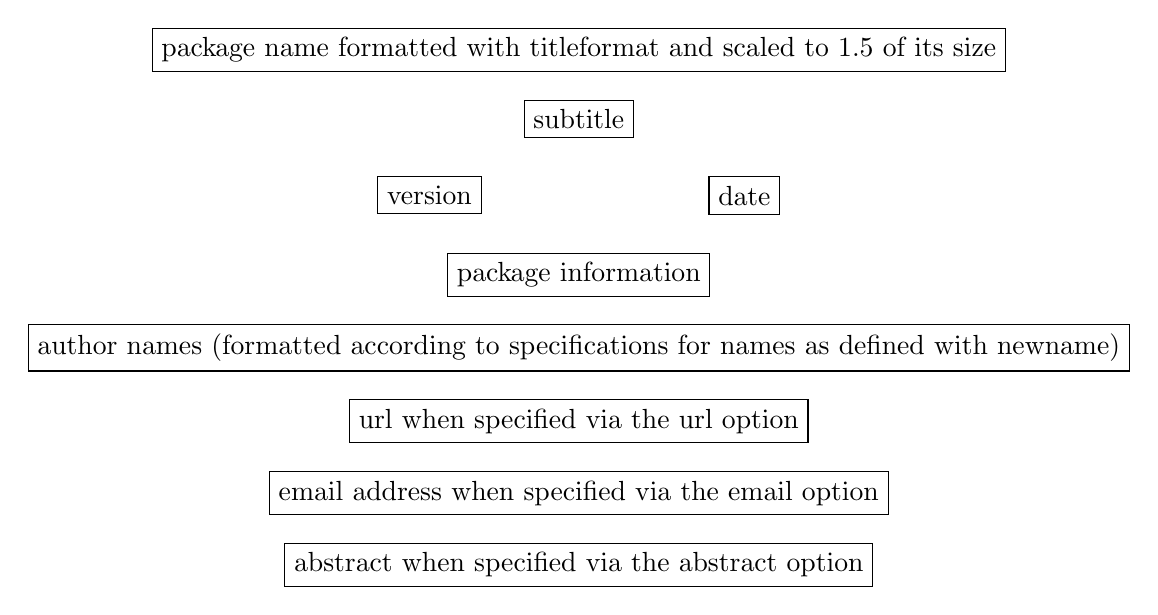
\begin{tikzpicture}[
      start chain=going below,
      node distance=1em,
      every node/.style={draw,align=center}
    ]
    \node[on chain] {package name formatted with \cs{titleformat} and scaled
      to 1.5 of its size} ;
    \node[on chain] {subtitle} ;
    \node[on chain,draw=none]
      {\tikz\draw (0,0) node[draw] {version} ++(4,0) node[draw] {date} ;} ;
    \node[on chain] {package information} ;
    \node[on chain] {author names (formatted according to specifications for
      names as defined with \cs{newname})} ;
    \node[on chain] {url when specified via the \option{url} option} ;
    \node[on chain] {email address when specified via the \option{email} option} ;
    \node[on chain] {abstract when specified via the \option{abstract} option} ;
  \end{tikzpicture}
  \caption{Schematic sketch of the title page.}
  \label{fig:titlepage}
\end{figure}

\subsection{A Quotation Environment}

\cnltxdoc\sinceversion{0.5} provides a quotation environment:
\begin{environments}
  \environment{cnltxquote}[\oarg{author/reference}]
    A quotation environment.
\end{environments}

The environment sets the body indented on both sides as it simply uses a
\env*{quote} environment internally.  The contents of the optional argument is
set flush right after the environment's body.  The formatting is controlled by
two options:

\begin{options}
  \keyval{quote-format}{definition}\Default{\cs*{small}\cs*{sffamily}}
    The formatting of the environment's body.
  \keyval{quote-author-format}{definition}\Default{\cs*{itshape}}
\end{options}

\begin{example}
  \begin{cnltxquote}[Douglas Adams, The Restaurant at the End of the Universe]
    ``The first ten million years were the worst,'' said Marvin, ``and the
    second ten million years, they were the worst too.  The third ten million
    years I didn't enjoy at all.  After that I went into a bit of a decline.''
  \end{cnltxquote}
\end{example}

\subsection{Predefined Preamble}\label{sec:preamble}
It is possible to load a part of my standard preamble automatically by
passing an option as class option.
\begin{options}
  \opt{load-preamble}
    Class option that preloads part of my custom preamble.
\end{options}

Using the option will include the following code:\changedversion{0.13}

\begin{sourcecode}
  \RequirePackage{ifxetex,ifluatex}
  \ifbool{cnltx@load@fonts}
    {
      \ifboolexpr{not bool{xetex} and not bool{luatex}}
        {\RequirePackage[T1]{fontenc}}
        {\RequirePackage{fontspec}}
      \RequirePackage[oldstyle]{libertine}
      \RequirePackage{libertinehologopatch}
      \RequirePackage[supstfm=libertinesups]{superiors}
      % libertine does not have superior letters:
      \def\@makefnmark{%
        \hbox{%
          \cnltx@ifisnum{\@thefnmark}
            {\textsu{\hspace*{\superiors@spaced}\@thefnmark}}
            {\@textsuperscript{\normalfont\@thefnmark}}%
        }%
      }
    }
    {}
  \ifbool{cnltx@microtype}
    {\RequirePackage{microtype}}
    {}
  \ifboolexpr
    {
      bool {cnltx@microtype} and
      not test {\ifcsdef{MT@pr@set@@romansans}} and
      not test {\ifcsdef{MT@ex@set@@romansans}} and
      bool {cnltx@load@fonts}
    }
    {
      \DeclareMicrotypeSet{romansans}{
        encoding = {*},
        family   = {rm*,sf*}
      }
    }
    {}
  \ifboolexpr
    {
      bool {cnltx@microtype} and
      not test {\ifcsdef{MT@tr@set@@scshape}} and
      bool {cnltx@load@fonts}
    }
    {
      \DeclareMicrotypeSet[tracking]{scshape}{
        encoding = {*} ,
        shape    = {sc,scit,si}
      }
    }
    {}
  \ifboolexpr
    {
      not bool {xetex} and
      bool {cnltx@load@fonts} and
      bool {cnltx@microtype}
    }
    {
      \microtypesetup{
        tracking   = scshape ,
        protrusion = romansans ,
        expansion  = romansans
      }
      \DisableLigatures{ family = tt* }
    }
    {}
  \ifbool{cnltx@load@fonts}
    {
      \ifboolexpr{not bool{xetex} and not bool{luatex}}
        {\RequirePackage[scaled=.81]{beramono}}
        {
          \setmonofont[
            Scale = MatchLowercase ,
            Ligatures = {NoCommon,NoRequired,NoContextual}
          ]{DejaVu Sans Mono}
        }
      \KOMAoptions{DIV=last}
      \recalctypearea
    }
    {}
  \RequirePackage{fnpct}
  \expandafter\RequirePackage\expandafter[\cnltx@babel@options]{babel}
\end{sourcecode}

The effect of this preamble is demonstrated by the document you're reading at
this moment.

\begin{options}
  \keybool{load-preamble-}\Default{false}
    This option has the same effect as adding using \option{load-preamble} but
    without making any font decisions.
\end{options}

Another option affects the layout of the document:
\begin{options}
  \keybool{adapt-layout}\Default{true}
    \sinceversion{0.13}If set to true \cnltxdoc\ will make some changes to the
    section and part formats, it will redefine the footnote format, set the
    header and footer and adapt the caption format.
\end{options}

Using the option will include the following code:

\begin{sourcecode}
  \renewcommand*\sectionformat{%
    \textcolor{cnltx}{\thesection\autodot}\enskip
  }
  \renewcommand*\subsectionformat{%
    \textcolor{cnltx}{\thesubsection\autodot}\enskip
  }
  \renewcommand*\subsubsectionformat{%
    \textcolor{cnltx}{\thesubsubsection\autodot}\enskip
  }
  \setkomafont{subsubsection}{\normalfont\normalsize\itshape}
  \renewcommand*\partformat{%
    \textcolor{cnltx}{\partname~\thepart\autodot}%
  }
  \renewcommand*\partformat{%
    \textcolor{cnltx}{\partname~\thepart\autodot}}
  \deffootnote{2em}{1em}{\llap{\thefootnotemark. }}%
  \RequirePackage{scrlayer-scrpage}
  \chead{\rightmark}
  \KOMAoptions{automark}
  \pagestyle{scrheadings}
  \setcapindent{1.5em}
  \setkomafont{caption}{\cnltx@caption@font}
  \setkomafont{captionlabel}{\cnltx@captionlabel@font}
\end{sourcecode}

\subsection{Predefined Indexing}\label{sec:predefined-indexing}
\cnltxdoc\ allows the automated creation of an index.  This is done with the
help of the \pkg{imakeidx} package by \egreg~\cite{pkg:imakeidx}.  To use this
feature you have two class options.  They cannot be set with \cs{setcnltx} but
must be given as class options.

\begin{options}
  \keybool{add-index}\Default{false}
    Enables the automatic creation of an index at the end of the document.
  \keybool{load-preamble+}\Default{false}
    This option has the same effect as adding the options
    \option{load-preamble}, \option{add-index} and \option{add-bib}.
\end{options}

Enabling the feature
\begin{itemize}
  \item loads the \needpackage{imakeidx} package,
  \item uses a given style file for the index that can be specified with the
    \option{index-style} option,
  \item sets a certain setup for the index that can be specified with the
    \option{index-setup} option and
  \item adds an index at the end of the document.
\end{itemize}

The following options are available to customize the appearance of the index:
\begin{options}
  \keyval{index-prologue}{text}
    Adds \meta{text} as index prologue between heading and the actual index.
  \keyval{index-space}{dimension}\Default{0pt}
    The vertical space between index prologue and index.
  \keyval{index-setup}{options}%
    \Default{othercode=\cs*{footnotesize},level=\cs*{addsec}}
    The options that are passed to \pkg{imakeidx}'s \cs*{indexsetup} command.
  \keyval{makeindex-setup}{options}\Default{columns=2,columnsep=1em}
    The options that are passed to the \cs*{makeindex} command.
  \keyval{index-style}{style file}\Default{cnltx.ist}
    The style file that is used for formatting the index.
\end{options}

The index style file \file{cnltx.ist} contains the following lines:
\inputsourcecode[sourcecode-options={style=cnltx-makeindex}]{cnltx.ist}

The feature is demonstrated by this document which does not contain a single
control sequence containing the string \code{index}!

\subsection{Bibliography with \pkg*{biblatex}}
\subsubsection{Bibliography Entry Types \code{package}, \code{class} and
  \code{bundle} for \pkg*{biblatex}}
\label{sec:listings:bibtex-language}

\cnltxdoc\sinceversion{0.4} defines the bibliograpy entry types
\code{package}, \code{class} and \code{bundle} when
\pkg{biblatex}~\cite{pkg:biblatex} is used.  This allows specifying \LaTeX\
packages in \file{bib} files:

\begin{sourcecode}[sourcecode-options={style=cnltx-bibtex}]
  @package{pkg:chngcntr,
    title      = {chngcntr} ,
    author     = {Peter Wilson} ,
    maintainer = {Will Robertson} ,
    date       = {2009-09-02} ,
    version    = {1.0a} ,
    url        = {http://mirror.ctan.org/macros/latex/contrib/chngcntr/}
  }
  @class{cls:exam,
    title      = {exam},
    author     = {Philip Hirschhorn},
    date       = {2015-05-07},
    version    = {2.5},
    url        = {http://mirror.ctan.org/macros/latex/contrib/exam/}
  }
  @bundle{bnd:koma-script,
    title          = {\KOMAScript} ,
    sorttitle      = {KOMA-Script} ,
    indextitle     = {\KOMAScript} ,
    indexsorttitle = {KOMA-Script} ,
    author         = {Markus Kohm},
    date           = {2015-07-02} ,
    version        = {3.18} ,
    url            = {http://mirror.ctan.org/macros/latex/contrib/koma-script/}
  }
\end{sourcecode}

As you can see also an entry field \code{maintainer} is defined.  For this to
work you have to use the \pkg{biblatex} bibliography style \code{cnltx}.  This
style basically is a clone of the style \code{alphabetic} but defines the
necessary additions for the \code{package}, \code{class} and \code{bundle}
entry types and the \code{maintainer} entry field.

Along with the bibliography style a citation style \code{cnltx} is provided,
again a clone of the \code{alphabetic} style.  The only addition it makes is
that indexing of maintainer names is enabled if \pkg{biblatex}'s
\code{indexing} option is used.  The styles load \cnltxexample\ as it relies
on definitions made by it.

This document uses the following call of \pkg{biblatex}:
\begin{sourcecode}
  \usepackage[
    backend=biber,
    style=cnltx,
    sortlocale=en_US,
    indexing=cite,
    useprefix]{biblatex}
  \addbibresource{cnltx.bib}
\end{sourcecode}
Actually it let's \cnltxdoc\ do it, see section~\ref{sec:autom-bibl} for
details.

Just for the sake of the example I am going to cite the \pkg*{chngcntr}
package now~\cite{pkg:chngcntr} so you can see both the bibliography entry and
the indexed names of package, author and maintainer in the appendix.

\subsubsection{Automatic Bibliography}\label{sec:autom-bibl}

\cnltxdoc\ allows the automated creation of a bibliography.

\begin{options}
  \keybool{add-bib}\Default{false}
    Enables the automatic creation of a bibliography at the end of the
    document.
  \keybool{load-preamble+}\Default{false}
    This option has the same effect as adding the options
    \option{load-preamble}, \option{add-index} and \option{add-bib}.
\end{options}

What this options does is including the following code:
\begin{sourcecode}
  \RequirePackage[
    backend=biber,
    style=cnltx,
    sortlocale=en_US,
    indexing=cite,
    useprefix]{biblatex}
  \addbibresource{cnltx.bib}
  \AtEndDocument{\printbibliography}
\end{sourcecode}

As you can see there's also a bibliography database file \file{cnltx.bib} that
provides a yet small but growing number of package entries.

\section{Predefined \pkg*{listings} and \pkg*{mdframed} Styles}
\subsection{\pkg*{mdframed}}

The source code environments (see section~\vref{sec:usage:examples}) all get a
frame with the help of the \pkg{mdframed}~\cite{pkg:mdframed} package.  For
this a custom style is defined called \code{cnltx}.  The options
\option{frame-options} and \option{add-frame-options} mentioned in
section~\vref{sec:usage:examples} manipulate this style.  It is predefined
with these values:

\begin{sourcecode}
  \def\cnltx@mdframed@options{
    backgroundcolor = cnltxbg ,
    linecolor       = cnltx ,
    roundcorner     = 5pt
  }
\end{sourcecode}

\subsection{\pkg*{listings}}
\subsubsection{\LaTeX\ Sourcecode}\label{sec:listings-sourcecode}

The code of the source code environments (see
section~\vref{sec:usage:examples}) is formatted with the help of the
\pkg{listings} package~\cite{pkg:listings}.  A \pkg{listings} style is defined
called \code{cnltx}.  The options \option{add-cmds}, \option{add-silent-cmds},
\option{add-envs}, \option{add-silent-envs}, \option{listings-options} and
\option{add-listings-options} manipulate this style.  It is predefined by
\cnltxexample\ as follows:

\begin{sourcecode}
  \def\cnltx@listings@style{
    language         = [AlLaTeX]TeX,
    alsolanguage     = [plain]TeX,
    basicstyle       = {\sourceformat},
    numbers          = left,
    numberstyle      = \tiny,
    xleftmargin      = 1em,
    numbersep        = .75em,
    gobble           = \cnltx@gobble ,
    columns          = fullflexible,
    literate         =
      {ä}{{\"a}}1
      {ö}{{\"o}}1
      {ü}{{\"u}}1
      {Ä}{{\"A}}1
      {Ö}{{\"O}}1
      {Ü}{{\"U}}1
      {ß}{{\ss}}1 ,
    breaklines       = true,
    keepspaces       = true,
    breakindent      = 1em,
    commentstyle     = \color{comment},
    keywordstyle     = \color{cs},
    deletetexcs      =
      {
        a,o,u,A,O,U,
        begin,
        center,
        description,document,
        end,enumerate,
        figure,flushleft,flushright,
        itemize,list,
        otherlanguage,
        table,tabu,tabular
      },
    deletekeywords   =
      {
        a,o,u,A,O,U,
        begin,
        center,
        description,document,
        end,enumerate,
        figure,flushleft,flushright,
        itemize,list,
        otherlanguage,
        table,tabu,tabular
      },
    % \begin, \end:
    texcsstyle       = [2]\color{beginend},
    index            = [2][texcs2],
    indexstyle       = [2]\@gobble,
    moretexcs        = [2]{begin,end},
    % added environments that'll be indexed:
    texcsstyle       = [3]\color{env},
    index            = [3][texcs3],
    indexstyle       = [3]\envidx,
    % environments that won't be indexed:
    texcsstyle       = [4]\color{env},
    index            = [4][texcs4],
    indexstyle       = [4]\@gobble,
    % control sequences that'll be indexed:
    texcsstyle       = [5]\color{cs},
    index            = [5][texcs5],
    indexstyle       = [5]\indexcs,
    % control sequences that won't be indexed:
    texcsstyle       = [6]\color{cs},
    index            = [6][texcs6],
    indexstyle       = [6]\@gobble
  }
\end{sourcecode}

\subsubsection{\BibTeX\ Entries}
The \cnltxlistings\ package defines\sinceversion{0.4} a \pkg{listings}
language \code{BibTeX} that contains a huge number of bibentry types and
bibentry field types, have a look at
section~\vref{sec:listings:bibtex-language}.  \cnltxexample\ defines a
\pkg{listings} style for formatting them called \code{cnltx-bibtex}:

\begin{sourcecode}
  \def\cnltx@bibtex@listings@style{
    language         = BiBTeX,
    basicstyle       = {\sourceformat},
    numbers          = left,
    numberstyle      = \tiny,
    xleftmargin      = 1em,
    numbersep        = .5em,
    gobble           = \cnltx@gobble ,
    columns          = fullflexible,
    literate         =
      {ä}{{\"a}}1
      {ö}{{\"o}}1
      {ü}{{\"u}}1
      {Ä}{{\"A}}1
      {Ö}{{\"O}}1
      {Ü}{{\"U}}1
      {ß}{{\ss}}1 ,
    breaklines       = true,
    keepspaces       = true,
    breakindent      = 1em,
    commentstyle     = \color{comment},
    keywordstyle     = \color{bibentry} ,
    keywordstyle     = [2]\color{bibentryfield}\itshape ,
    showstringspaces = false ,
  }
\end{sourcecode}

\subsubsection{\code{makeindex} Style Files}
\cnltxlistings\ defines\sinceversion{0.7} a \pkg{listings} language
\code{makeindex} that contains the keywords used in \code{makeindex} style
files.  \cnltxexample\ defines a \pkg{listings} style for formatting them
called \code{cnltx-makeindex}:

\begin{sourcecode}
  \def\cnltx@makeindex@listings@style{
    language         = makeindex,
    basicstyle       = {\sourceformat},
    numbers          = left,
    numberstyle      = \tiny,
    xleftmargin      = 1em,
    numbersep        = .75em,
    gobble           = \cnltx@gobble ,
    columns          = fullflexible,
    literate         =
      {ä}{{\"a}}1
      {ö}{{\"o}}1
      {ü}{{\"u}}1
      {Ä}{{\"A}}1
      {Ö}{{\"O}}1
      {Ü}{{\"U}}1
      {ß}{{\ss}}1 ,
    breaklines       = true,
    keepspaces       = true,
    breakindent      = 1em,
    commentstyle     = \color{comment},
    keywordstyle     = \color{makeidxkey}\bfseries ,
    stringstyle      = \color{makeidxstring} ,
    showstringspaces = false
  }
\end{sourcecode}

\section{\PDF\ Strings and \pkg*{hyperref}}

Since the formatting and indexing commands \cs{cs}, \cs{env}, \cs{option},
\cs{pkg}, \cs{cls} and \cs{key} are robust they are ignored in \PDF\
strings.  For this reason you should \emph{only use the starred variants} in
places where \PDF\ bookmarks are built from such as section titles when you
use \pkg{hyperref}~\cite{pkg:hyperref}.  Since \cnltxdoc\ loads \pkg{hyperref}
this means you should do so, too, when you use \cnltxdoc.  This is important
for two reasons:
\begin{enumerate}
  \item Indexing in strings that get written to the table of contents does
    noch make much sense, anyway, so the starred versions should be used in
    section titles even if you don't use \pkg{hyperref}.
  \item When \pkg{hyperref} is loaded the mentioned commands are disabled in
    \PDF\ strings in a way that \emph{expects} them to be followed by a star.
    This means leaving the star out will result in \code{doesn't match its
      definition} errors.
\end{enumerate}

\section{Predefined Colors and Color-Schemes}\label{sec:colors}
\subsection{Explicitly Defined Colors}\label{sec:expl-defin-colors}

The \cnltxbase\ package defines a number of colors:
\begin{colors}
  \colour{cnltxbrown}
    Per default used for the control sequences.
  \colour{cnltxblue}
    Per default used for module names.
  \colour{cnltxred}
    Per default used as base color in various places.
  \colour{cnltxgreen}
    Unused per default.
  \colour{cnltxgray}
    Per default used for formatting comments.
  \colour{cnltxyellow}
    Per default used for option names.
  \colour{cnltxformalblue}
    Unused per default.
  \colour{cnltxformalred}
    Unused per default.
\end{colors}

\subsection{Actual Used Color Names and Color Schemes}\label{sec:actual-used-color}

The colors defined in section~\vref{sec:expl-defin-colors} are not directly
used with those names.  Instead colors are used whose names describe their
function rather than the color.  For this the color names are mapped to actual
colors and saved as a coloring scheme.  There are currently three predefined
color schemes whose definitions are given below.  Those definitions also show
the actually used color names.  They are defined via the following command:

\begin{commands}
  \command{definecolorscheme}[\marg{name}\marg{color assignments}]
    \sinceversion{0.5}Defines the color scheme \meta{name}.  When used all
    assignments will be actually carried out with \pkg{xcolor}'s
    \cs*{colorlet} command.  How to input \meta{color assignments} will be
    immediately clear from the examples below.
\end{commands}

To activate a color scheme for a document it is simply selected through an
option:
\begin{options}
  \keyval{color-scheme}{color scheme name}\Default{default}
    Activate a color scheme previously defined with \cs{definecolorscheme}.
\end{options}

The `default' color scheme is defined as follows:
\begin{sourcecode}
  \definecolorscheme{default}{
    cs            => cnltxbrown , % command sequences
    option        => cnltxyellow ,% options
    module        => cnltxblue ,  % modules
    comment       => cnltxgray ,  % comments
    beginend      => red ,        % \begin and \end
    env           => black ,      % environment names
    argument      => black ,      % argument delimiters
    meta          => black!80 ,   % arguments of \meta
    cnltx         => cnltxred ,   % base color
    cnltxbg       => white ,      % source code box background
    link          => black!90 ,   % hyperlinks
    versionnote   => black!75     % versioning notes text
    bibentry      => cnltxgreen , % BibTeX entry types
    bibentryfield => black,       % BibTeX entry fields
    expandable    => red ,        % the color used in \expandable
    unexpandable  => black ,      % the color used in \unexpandable
    makeidxkey    => cnltxgreen , % used for keywords in the cnltx-makeindex
                                  % style
    makeidxstring => black        % used for strings in the cnltx-makeindex
                                  % style 
  }
\end{sourcecode}

The `blue' color scheme is defined this way:
\begin{sourcecode}
  \definecolorscheme{blue}{
    cs            => cnltxbrown ,
    option        => cnltxgreen ,
    module        => cnltxred ,
    comment       => cnltxgray ,
    beginend      => red ,
    env           => black ,
    argument      => black ,
    meta          => black!80 ,
    cnltx         => cnltxblue ,
    cnltxbg       => yellow!10 ,
    link          => cnltx ,
    versionnote   => black!75
    bibentry      => cnltxyellow ,
    bibentryfield => black ,
    expandable    => red ,
    unexpandable  => black ,
    makeidxkey    => cnltxyellow ,
    makeidxstring => black
  }
\end{sourcecode}

Finally the `formal' color scheme is defined like this:
\begin{sourcecode}
  \definecolorscheme{formal}{
    cs            => black ,
    option        => cnltxformalblue ,
    module        => cnltxblue ,
    comment       => cnltxgray ,
    beginend      => red ,
    env           => black ,
    argument      => black ,
    meta          => black!80 ,
    cnltx         => cnltxformalblue ,
    cnltxbg       => white ,
    link          => black!90 ,
    versionnote   => black!75 ,
    bibentry      => black ,
    bibentryfield => black ,
    expandable    => red ,
    unexpandable  => black ,
    makeidxkey    => black ,
    makeidxstring => black
  }
\end{sourcecode}

\section{Language Support}\label{sec:language-support}
\noindent\sinceversion{0.2}The \cnltxdoc, the \cnltxexample\ and the
\cnltxtools\ package as well as the \code{cnltx.ist} index style and the
\code{cnltx} \pkg{biblatex} style all rely on the \pkg{translations}
package~\cite{pkg:translations} for providing some document language dependent
strings\footnote{Actually they depend on \cnltxtranslations\ which in turn
  loads \pkg{translations}.}.  Currently only translations for English and
German are provided.  Others can be added and the existing ones changed with
the following commands provided by the \pkg{translations} package:

\begin{commands}
  \command{DeclareTranslation}[\marg{language}\marg{keyword}\marg{translation}]
    Define or redefine translations for the string identified by the
    \textsc{id} \meta{keyword}.
  \command{RenewTranslation}[\marg{language}\marg{keyword}\marg{translation}]
    Renew translations for the string identified by the \textsc{id}
    \meta{keyword}.
\end{commands}

The strings defined by \cnltx\ are listed in
table~\vref{tab:language:strings}.  They are used in indexing strings and in
different parts of the document.

\begin{table}
  \centering\renewcommand\arraystretch{1.3}
  \caption{Overview over available internationalization key words.}
  \label{tab:language:strings}
  \begin{tabular}{
      l
      >{\ttfamily}l
      >{\RaggedRight}p{.25\linewidth}
      >{\RaggedRight}p{.25\linewidth}
    }
    \toprule
      Package/Class & key word          & English version & German version\\
    \midrule
      \cnltxexample & cnltx-package &
        \GetTranslation{cnltx-package} &
        \GetTranslationFor{German}{cnltx-package} \\
      \cnltxexample & cnltx-class &
        \GetTranslation{cnltx-class} &
        \GetTranslationFor{German}{cnltx-class} \\
      \cnltxexample & cnltx-bundle &
        \GetTranslation{cnltx-bundle} &
        \GetTranslationFor{German}{cnltx-bundle} \\
      \cnltxexample & cnltx-environment &
        \GetTranslation{cnltx-environment} &
        \GetTranslationFor{German}{cnltx-environment} \\
      \cnltxdoc     & cnltx-default &
        \GetTranslation{cnltx-default} &
        \GetTranslationFor{German}{cnltx-default} \\
      \cnltxdoc     & cnltx-empty &
        \GetTranslation{cnltx-empty} &
        \GetTranslationFor{German}{cnltx-empty} \\
      \cnltxdoc     & cnltx-required &
        \GetTranslation{cnltx-required} &
        \GetTranslationFor{German}{cnltx-required} \\
      \cnltxdoc     & cnltx-toc &
        \GetTranslation{cnltx-toc} &
        \GetTranslationFor{German}{cnltx-toc} \\
      \cnltxdoc     & cnltx-license &
        \GetTranslation{cnltx-license} &
        \GetTranslationFor{German}{cnltx-license}\\
      \cnltxdoc     & cnltx-introduced &
        \GetTranslation{cnltx-introduced} &
        \GetTranslationFor{German}{cnltx-introduced} \\
      \cnltxdoc     & cnltx-changed &
        \GetTranslation{cnltx-changed} &
        \GetTranslationFor{German}{cnltx-changed} \\
      \cnltxdoc     & cnltx-f. &
        \GetTranslation{cnltx-f.} &
        \GetTranslationFor{German}{cnltx-f.} \\
      \cnltxdoc     & cnltx-ff. &
        \GetTranslation{cnltx-ff.} &
        \GetTranslationFor{German}{cnltx-ff.} \\
      \cnltxdoc     & cnltx-maintainer &
        \GetTranslation{cnltx-maintainer} &
        \GetTranslationFor{German}{cnltx-maintainer} \\
      \cnltxdoc     & cnltx-maintainers &
        \GetTranslation{cnltx-maintainers} &
        \GetTranslationFor{German}{cnltx-maintainers} \\
      \cnltxtools   & cnltx-i.e. &
        \GetTranslation{cnltx-i.e.} &
        \GetTranslationFor{German}{cnltx-i.e.} \\
      \cnltxtools   & cnltx-e.g. &
        \GetTranslation{cnltx-e.g.} &
        \GetTranslationFor{German}{cnltx-e.g.} \\
      \cnltxtools   & cnltx-cf. &
        \GetTranslation{cnltx-cf.} &
        \GetTranslationFor{German}{cnltx-cf.} \\
      \cnltxtools   & cnltx-etc. &
        \GetTranslation{cnltx-etc.} &
        \GetTranslationFor{German}{cnltx-etc.} \\
    \bottomrule
  \end{tabular}
\end{table}

\part{Appendix}
\appendix

\section{Internal Helper Commands}

The commands in this section are only described for the sake of completeness.
They are not meant to be used in a document.  Some of them might be useful in
\LaTeX\ programming, though.  Expandable commands are marked with
\textcolor{expandable}{\expandablesign}.

\subsection{Defined by \cnltxbase}\label{sec:defined-cnltxbase}

Especially \cnltxbase\ defines some useful helper macros that are also used by
the other packages and classes.

\subsubsection{Related to the Bundle}\label{sec:related-bundle}

\begin{commands}
  \expandable\command{cnltx\at\at date}
    The creation date of the current version of the bundle.
  \expandable\command{cnltx\at\at version}
    The version number of the bundle.
  \expandable\command{cnltx\at\at info}
    The short description of the bundle.
  \command{cnltx\at create\at bundle\at message}%
    [\sarg\marg{module}\Marg{\choices{Error,Warning,WarningNoLine,Info}}]
    \sinceversion{0.7}Create suiting error and warning messaging commands
    for the module \meta{module} of the \cnltx\ bundle.  The starred version
    creates messages for a class the un-starred version messages for a
    package.
  \command{cnltx\at base\at error}[\marg{message}]
    Issue an error message using \cs*{PackageError}\Marg{cnltx-base}.
  \command{cnltx\at base\at warning}[\marg{message}]
    Issue a warning message using \cs*{PackageWarning}\Marg{cnltx-base}.
    \command{cnltx\at base\at warningnoline}[\marg{message}]
    Issue a warning message using \cs*{PackageWarningNoLine}\Marg{cnltx-base}.
  \command{cnltx\at base\at info}[\marg{message}]
    Issue a message using \cs*{PackageInfo}\Marg{cnltx-base}.
  \command{cnltx\at define\at colorscheme}[\marg{name}\marg{scheme definition}]
    Command that can be used to define a color scheme.
  \command{cnltx\at load\at module}[\marg{\cnltx\ module}]
    \sinceversion{0.11}Loads the package \code{cnltx-\meta{\cnltx\
        module}.sty}.
  \command{cnltx\at load\at modules}[\marg{\cnltx\ modules}]
    \sinceversion{0.11}Maps the comma separated list \meta{\cnltx\ modules} to
    \cs{cnltx\at load\at module}, leading and trailing spaces are trimmed.
\end{commands}

\subsubsection{Programming Tools}
\paragraph{Message Handling}
\begin{commands}
  \command{cnltx\at create\at message}%
    [\sarg\marg{prefix}\marg{package/class
      name}\Marg{\choices{Error,Warning,WarningNoLine,Info}} \marg{detailed
      error message}]
    \changedversion{0.7}Create error and warning messaging commands
    \cs*{\meta{prefix}@\choices{error,warning,warningnoline,info}}\marg{message}.
    The starred version creates messages for a class the un-starred version
    messages for a package.  All commands have one argument which takes the
    message.  \meta{prefix} will be all lowercase in the generated command.
  \command{cnltx\at create\at generic\at message}%
    [\sarg\marg{prefix}\marg{package/class
      name}\Marg{\choices{Error,Warning,WarningNoLine,Info}}]
    \sinceversion{0.7}Create error and warning messaging commands
    \cs*{\meta{prefix}@\choices{error,warning,warningnoline,info}}\marg{message}.
    The starred version creates messages for a class the un-starred version
    messages for a package.  All commands have one argument which takes the
    message \emph{except for the error command which gets two arguments}, the
    first for the short version and the second for the detailed message.
    \meta{prefix} will be all lowercase in the generated command.
\end{commands}

\paragraph{Conditionals}
\begin{commands}
  \expandable\command{iftest}[\marg{test directive}\marg{true}\marg{false}]
    \sinceversion{0.7}Checks if \meta{test directive} is true and either
    places \meta{true} or \meta{false} in the input stream.  \meta{test
      directive} should be a \TeX\ test like
    \cs*{ifx}\meta{token1}\meta{token2}, \ie, demand an \cs*{else} and
    \cs*{fi}.\\
    This is a command in the spirit of \pkg{etoolbox}'s \cs*{ifbool} that does
    the same for a boolean \meta{bool} defined with
    \cs*{newif}\cs*{if\meta{bool}} or \cs*{newbool}\marg{bool}.  It
    corresponds to \pkg{etoolbox}'s \code{test} directive for its
    \cs*{ifboolexpr}.
  \expandable\command{nottest}[\marg{test directive}\marg{not true}\marg{not false}]
    \sinceversion{0.7}Checks if \meta{test directive} is not true and either
    places \meta{not true} or \meta{not false} in the input stream.  Test
    directive should be a \TeX\ test like
    \cs*{ifx}\meta{token1}\meta{token2}, \ie, demand an \cs*{else} and
    \cs*{fi}.\\
    This is a command in the spirit of \pkg{etoolbox}'s \cs*{notbool} that does
    the same for a boolean \meta{bool} defined with
    \cs*{newif}\cs*{if\meta{bool}} or \cs*{newbool}\marg{bool}.
  \expandable\command{cnltx\at ifcounter}[\marg{counter}\marg{true}%
    \marg{false}]
    \sinceversion{0.11}Checks if \meta{counter} is a counter, \ie, if the
    control sequence names \cs*{c@\meta{counter}}, \cs*{cl@\meta{counter}},
    \cs*{p@\meta{counter}} \emph{and} \cs*{the\meta{counter}} exist and either
    leaves \meta{true} or \meta{false} in the input stream.
  \command{cnltx\at ifnextchars}[\marg{list of
    tokens}\marg{true}\marg{false}\meta{trailing token}]
    \sinceversion{0.8}Tests if \meta{trailing token} is any of those in
    \meta{list of tokens} and either places \meta{true} or \meta{false} in the
    input stream without removing \meta{trailing token}.
  \command{cnltx\at ifsym}[\marg{token}\marg{true}\marg{false}]
    A generic version of \LaTeX's \cs*{@ifstar} that checks if \meta{token}
    follows in the input stream.  If yes it is removed and \meta{true} is
    placed in the input stream else \meta{false}.
  \command{cnltx\at ifdash}[\marg{true}\marg{false}]
    A wrapper for \verbcode+\cnltx@ifsym{-}+.
  \command{cnltx\at ifbang}[\marg{true}\marg{false}]
    \sinceversion{0.3}A wrapper for \verbcode+\cnltx@ifsym{!}+.
  \expandable\command{cnltx\at ifisnum}[\marg{token list}\marg{true}\marg{false}]
    \sinceversion{0.6}Checks if \meta{token list} is an integer zero or
    greater and leaves \meta{true} in the input stream if it is and
    \meta{false} if it isn't.  There is one hopefully extremely unlikely case
    where the test fails: when \meta{token list} starts with
    ``\code{\meta{integer}\%}'' where \code{\%} has a category code different
    than 9 (ignored) or 14 (comment).
  \expandable\command{cnltx\at ifshellescape}[\marg{true}\marg{false}]
    \sinceversion{0.9}Checks if shellescape is enabled.  It returns true if
    \pkg{pdftexcmds}' \cs*{pdf@shellescape} has the value~\code{1}.  This is a
    wrapper for \verbcode+\iftest{\ifnum\pdf@shellescape=1 }+.
  \command{cnltx\at if\at in}[\marg{tokenlist}\marg{search}\marg{true}\marg{false}]
    Places \meta{true} in the input stream if \meta{search} is found in
    \meta{tokenlist} and \meta{false} if it isn't.
  \expandable\command{cnltx\at ifstrequal}[\marg{string1}\marg{string2}%
    \marg{true}\marg{false}]
    \sinceversion{0.10}Tests if \meta{string1} is equal to \meta{string2} and
    either leaves \meta{true} or \meta{false} in the input stream.  This test
    doesn't take category codes into account.
  \command{cnltx\at ifinlist}%
    [\marg{item}\marg{listmacro}\marg{true}\marg{false}]
    \sinceversion{0.10}A conditional for \pkg{etoolbox} lists similar to
    \cs*{ifinlist} where braces in items are allowed.  This wraps around the
    proposal in \pkg{etoolbox}'s documentation to redefine \cs*{do} and loop
    through the list.
  \command{cnltx\at ifinlistcs}%
    [\marg{item}\marg{listcsname}\marg{true}\marg{false}]
    \sinceversion{0.10}A conditional for \pkg{etoolbox} lists similar to
    \cs*{ifinlistcs} where braces in items are allowed.  This wraps around the
    proposal in \pkg{etoolbox}'s documentation to redefine \cs*{do} and loop
    through the list.
\end{commands}

\paragraph{Expansion Tools}
\begin{commands}
  \command{expandtwice}[\marg{code}]
    \sinceversion{0.10}Expands \meta{code} twice in an \cs*{edef}-like
    context.  This is a  wrapper for\newline
    \cs*{unexpanded}\cs*{expandafter}\cs*{expandafter}\cs*{expandafter}.
  \command{cnltx\at expandargs}[\darg{specs}\meta{control sequence}]
    \sinceversion{0.7}This is a \LaTeXe\ version of expl3's
    \cs*{exp\_args:N}\meta{specs}.  The command expands the arguments of
    \meta{control sequence} according to \meta{specs}.  In \meta{specs}
    \begin{itemize}
      \item \code{N} means unexpanded token,
      \item \code{n} means unexpanded braced group,
      \item \code{c} means braced group converted into a control sequence
        name,
      \item \code{o} means braced group expanded once,
      \item \code{f} means braced group expanded with \cs*{romannumeral}, and
      \item \code{x} means braced group expanded with \cs*{edef}.
    \end{itemize}
\end{commands}

\paragraph{Category Code Stuff}
\begin{commands}
  \command{cnltx\at save\at catcode}[\marg{token}]
    \sinceversion{0.11}Saves the current category code of \meta{token}.
  \command{cnltx\at restore\at catcode}[\marg{token}]
    \sinceversion{0.11}Restores the category code of \meta{token} as
    previously saved with \cs{cnltx\at save\at catcode}.
  \command{cnltx\at set\at catcode}[\marg{token}\marg{catcode}]
    \sinceversion{0.11}Sets the category code of \meta{token} to
    \meta{catcode}.  This is a wrapper for \newline
    \code{\cs*{catcode}`\meta{token}=\meta{catcode}\cs*{relax}}.
  \command{cnltx\at save\at catcodes}[\marg{tokenlist}]
    \sinceversion{0.11}Maps \cs{cnltx\at save\at catcode} to all tokens in
    \meta{tokenlist}.
  \command{cnltx\at restore\at catcodes}[\marg{tokenlist}]
    \sinceversion{0.11}Maps \cs{cnltx\at restore\at catcode} to all tokens in
    \meta{tokenlist}.
  \command{cnltx\at set\at catcodes}[\marg{tokenlist}\marg{catcode}]
    \sinceversion{0.11}Maps \cs{cnltx\at set\at catcode} to all tokens in
    \meta{tokenlist}, \ie, all tokens get category code \meta{catcode}.
  \command{cnltx\at make\at letter}[\marg{token}]
    \sinceversion{0.11}A wrapper for \cs{cnltx\at set\at
      catcode}\marg{token}\Marg{11}.
  \command{cnltx\at make\at other}[\marg{token}]
    \sinceversion{0.11}A wrapper for \cs{cnltx\at set\at
      catcode}\marg{token}\Marg{12}.
  \command{cnltx\at make\at active}[\marg{token}]
    \sinceversion{0.11}A wrapper for \cs{cnltx\at set\at
      catcode}\marg{token}\Marg{13}.
\end{commands}

\paragraph{Token List Manipulation}
\begin{commands}
  \command{cnltx\at replace\at once}[\marg{cs}\marg{search}\marg{replace}]
    Replaces the first occurence of \meta{search} in the first expansion of
    \meta{cs} with \meta{replace}.
  \command{cnltx\at greplace\at once}[\marg{cs}\marg{search}\marg{replace}]
    \sinceversion{0.9}The same as \cs{cnltx\at replace\at once} but acts
    globally.
  \command{cnltx\at replace\at all}[\marg{cs}\marg{search}\marg{replace}]
    Replaces all occurences of \meta{search} in the first expansion of
    \meta{cs} with \meta{replace}.
  \command{cnltx\at greplace\at all}[\marg{cs}\marg{search}\marg{replace}]
    \sinceversion{0.9}The same as \cs{cnltx\at replace\at all} but acts
    globally.
  \command{cnltx\at remove\at once}[\marg{cs}\marg{search}]
    \sinceversion{0.3}Removes the first occurence of \meta{search} in the
    first expansion of \meta{cs}.
  \command{cnltx\at gremove\at once}[\marg{cs}\marg{search}]
    \sinceversion{0.9}The same as \cs{cnltx\at remove\at once} but acts
    globally.
  \command{cnltx\at remove\at all}[\marg{cs}\marg{search}]
    \sinceversion{0.3}Removes all occurences of \meta{search} in the first
    expansion of \meta{cs}.
  \command{cnltx\at gremove\at all}[\marg{cs}\marg{search}]
    \sinceversion{0.9}The same as \cs{cnltx\at remove\at all} but acts
    globally.
\end{commands}

\paragraph{Miscellaneous}
\begin{commands}
  \expandable\command{cnltx\at par}
    Expands to \cs*{par}.  Sometimes you need to smuggle a \cs*{par} in a
    short macro \ldots
  \expandable\command{cnltx\at stripbs}
    A shortcut for \verbcode+\expandafter\@gobble\string+.
  \command{cnltxat}
    Robust command that typesets `\at' with category code 11.  An @ in command
    names confuses the indexing of the command names.  Either one uses another
    symbol for makeindex's ``actual'' recognition and also tells
    \pkg{idxcmds}~\cite{pkg:idxcmds} about it or one uses \cs{cnltxat} in
    \cs{cs} and friends.  For the sake of convenience you can define a command
    like \cs*{at} that expands to it\footnote{This is important.  If you
      \cs*{let} it to \cs{cnltxat} index entries may be sorted differently!
      Remember: \cs{cnltxat} is robust.}.  In order not to overwrite any such
    existing macro it is not defined by \cnltxexample.  This document for
    example defines \verbcode+\def\at{\cnltxat}+.
  \command{cnltxletterat}
    An alias of \cs{cnltxat}.
  \command{cnltxotherat}
    The same as \cs{cnltxat} but with a `\at' with category code 12.
  \command{cnltxbang}
    The same as \cs{cnltxotherat} except that it contains a `\bang'.
  \command{cnltxequal}
    The same as \cs{cnltxotherat} except that it contains a `\equal'.
\end{commands}

\subsection{Defined by \cnltxdoc}
\begin{commands}
  \command{cnltx\at doc\at error}[\marg{message}]
    Issue an error message using \cs*{ClassError}\Marg{cnltx-doc}.
  \command{cnltx\at doc\at warning}[\marg{message}]
    Issue a warning message using \cs*{ClassWarning}\Marg{cnltx-doc}.
    \command{cnltx\at doc\at warningnoline}[\marg{message}]
    Issue a warning message using \cs*{ClassWarningNoLine}\Marg{cnltx-doc}.
  \command{cnltx\at doc\at info}[\marg{message}]
    Issue a message using \cs*{ClassInfo}\Marg{cnltx-doc}.
  \command{cnltx\at getfileinfo}[\marg{file name}\marg{file extension}]
    Extract the date, version and background information for a package or a
    class and defines \cs{cnltx\at package\at date}, \cs{cnltx\at package\at
      version} and \cs{cnltx\at package\at info} to contain the extracted
    data.
  \command{cnltx\at version\at note}[\marg{note}]
    Command that is used for the versioning notes interally.  Sets
    \cs*{reversemarginpar} and then writes the note \meta{note} to the margin
    with corresponding formatting.
\end{commands}
\begin{environments}
  \environment{cnltxlist}
    The list environment that is used by the environments \env{commands},
    \env{options} and \env{environments}.
\end{environments}

\subsection{Defined by \cnltxexample}
\begin{commands}
  \command{cnltx\at example\at error}[\marg{message}]
    Issue an error message using \cs*{PackageError}\Marg{cnltx-example}.
  \command{cnltx\at example\at warning}[\marg{message}]
    Issue a warning message using \cs*{PackageWarning}\Marg{cnltx-example}.
    \command{cnltx\at example\at warningnoline}[\marg{message}]
    Issue a warning message using \cs*{PackageWarningNoLine}\Marg{cnltx-example}.
  \command{cnltx\at example\at info}[\marg{message}]
    Issue a message using \cs*{PackageInfo}\Marg{cnltx-example}.
  \command{cnltx\at isvalue}
    Used in definitions of the key/value option typesetting commands.  Inserts
    a \code{=} with some stretchable space around and a legal break-point
    after it.
  \command{indexcs}
    Version of \cs{csidx} that takes care of a \cs*{textcompwordmark} inserted
    by listings. Also replaces all occurences of @ with category code 11 or 12
    with \cs{cnltxat}. Used to index commands in the \env{sourcecode} and
    \env{example} environments that have been added with \option{add-cmds}.
  \command{indexenv}
    \sinceversion{0.7a}Version of \cs{envidx} that takes care of a
    \cs*{textcompwordmark} inserted by listings. Also replaces all occurences
    of @ with category code 11 or 12 with \cs{cnltxat}. Used to index
    environments in the \env{sourcecode} and \env{example} environments that
    have been added with \option{add-envs}.
  \command{cnltx\at treat\at lst\at index}[\marg{new index cs}\marg{internal
    index cs}]
    \sinceversion{0.7a}This command was used to define \cs{indexcs} and
    \cs{indexenv}:\\
    \verbcode+\cnltx@treat@lst@index{\indexcs}{\csidx}+
  \command{MakePercentComment}
    Sets the category code of \code{\%} to 14.
  \command{cnltx\at copyablespace}
    Prints a space that is also copyable.  Uses the \pkg{accsupp} package by
    \oberdiek~\cite{pkg:accsupp}.
  \command{cnltx\at mdframed\at options}
    Predefined option list for the \pkg{mdframed}~\cite{pkg:mdframed} style
    \code{cnltx}.
  \command{cnltx\at listings\at style}
    Predefined option list for the \pkg{listings}~\cite{pkg:listings} style
    \code{cnltx}.
\end{commands}

\subsection{Defined by \cnltxlistings}
\begin{commands}
  \command{cnltx\at listings\at error}[\marg{message}]
    Issue an error message using \cs*{PackageError}\Marg{cnltx-listings}.
  \command{cnltx\at listings\at warning}[\marg{message}]
    Issue a warning message using \cs*{PackageWarning}\Marg{cnltx-listings}.
    \command{cnltx\at listings\at warningnoline}[\marg{message}]
    Issue a warning message using \cs*{PackageWarningNoLine}\Marg{cnltx-listings}.
  \command{cnltx\at listings\at info}[\marg{message}]
    Issue a message using \cs*{PackageInfo}\Marg{cnltx-listings}.
  \command{cnltx\at predefined\at control\at sequences}
    A comma-separated list of predefined `silent' control sequence names.
  \command{cnltx\at predefined\at environments}
    A comma-separated list of predefined `silent' environment names.
  \command{listsilentcmds}
    Prints all known control sequence names formatted and separated with the
    separator set with \option{list-sep}.  Requires \cnltxexample.
  \command{listsilentenvs}
    Prints all known environment names formatted and separated with the
    separator set with \option{list-sep}.  Requires \cnltxexample.
  \command{listbibfilekeys}[\marg{file name}]
    \sinceversion{0.7}Prints all cite keys contained in the bibliography file
    \meta{file name} formatted with \cs{code} and separated with the
    separator set with \option{list-sep}.  Requires \cnltxexample.
  \command{listbibfiletypes}[\marg{file name}]
    \sinceversion{0.7}Prints all citation types contained in the bibliography
    file \meta{file name} formatted with \cs{code} and separated with the
    separator set with \option{list-sep}.  Requires \cnltxexample.
  \command{listbibfileentries}[\marg{file name}]
    \sinceversion{0.7}Prints all cite keys contained in the bibliography file
    \meta{file name} formatted  with \cs{code} and gives their respective
    entry types, separated with the separator set with \option{list-sep}.
    Requires \cnltxexample.
\end{commands}
\begin{options}
  \keyval{list-sep}{separator}\Default{,\cs*{space}}
    Sets the separator for \cnltxlistings' commands listing the different
    commands \etc.
\end{options}

\subsection{Defined by \cnltxtools}
\begin{commands}
  \command{cnltx\at tools\at error}[\marg{message}]
    Issue an error message using \cs*{PackageError}\Marg{cnltx-tools}.
  \command{cnltx\at tools\at warning}[\marg{message}]
    Issue a warning message using \cs*{PackageWarning}\Marg{cnltx-tools}.
    \command{cnltx\at tools\at warningnoline}[\marg{message}]
    Issue a warning message using \cs*{PackageWarningNoLine}\Marg{cnltx-tools}.
  \command{cnltx\at tools\at info}[\marg{message}]
    Issue a message using \cs*{PackageInfo}\Marg{cnltx-tools}.
  \command{cnltx\at accsupp}[\marg{actual text}\marg{additional
    options}\marg{\TeX\ text}]
    A wrapper for package \pkg{accsupp}'s\newline
    \cs*{BeginAccSupp}\Marg{ActualText = \meta{actual text}}\meta{\TeX\ text}%
    \cs*{EndAccSupp}\marg{}.
\end{commands}

\section{List of Known \LaTeX\ Control Sequences}\label{sec:known:csnames}

Below all \emph{predefined} control sequence names are listed that are treated
as ``silent'' names by \cnltx, that is, those defined by \cnltxlistings.

\begin{multicols}{3}\small
  \RaggedRight\listsilentcmds
\end{multicols}

\section{List of Known \LaTeX\  Environments}\label{sec:known:environments}

Below all \emph{predefined} environment names are listed that are treated as
``silent'' names by \cnltx, that is, those defined by \cnltxlistings.

\begin{multicols}{3}\small
  \RaggedRight\listsilentenvs
\end{multicols}

\section{List of Entries in \code{cnltx.bib}}\label{sec:list-entr-bib}
Most entries in \code{cnltx.bib} are entries of the \code{@package} type.
The cite keys that the file currently contains are listed below.  This list is
very likely to be extended significantly in the future.

\setcnltx{list-sep={,\par}}
\begin{multicols}{3}\small
  \RaggedRight\listbibfileentries{cnltx.bib}
\end{multicols}

\end{document}
